\documentclass[compress]{beamer}
\usepackage{ifthen,verbatim}

\newcommand{\isnote}{}
\xdefinecolor{lightyellow}{rgb}{1.,1.,0.25}
\xdefinecolor{darkblue}{rgb}{0.1,0.1,0.7}

%% Uncomment this to get annotations
%% \def\notes{\addtocounter{page}{-1}
%%            \renewcommand{\isnote}{*}
%% 	   \beamertemplateshadingbackground{lightyellow}{white}
%%            \begin{frame}
%%            \frametitle{Notes for the previous page (page \insertpagenumber)}
%%            \itemize}
%% \def\endnotes{\enditemize
%% 	      \end{frame}
%%               \beamertemplateshadingbackground{white}{white}
%%               \renewcommand{\isnote}{}}

%% Uncomment this to not get annotations
\def\notes{\comment}
\def\endnotes{\endcomment}

\setbeamertemplate{navigation symbols}{}
\setbeamertemplate{headline}{\mbox{ } \hfill
\begin{minipage}{5.5 cm}
\vspace{-0.75 cm} \small
\end{minipage} \hfill
\begin{minipage}{4.5 cm}
\vspace{-0.75 cm} \small
\begin{flushright}
\ifthenelse{\equal{\insertpagenumber}{1}}{}{Jim Pivarski \hspace{0.2 cm} \insertpagenumber\isnote/\pageref{numpages}}
\end{flushright}
\end{minipage}\mbox{\hspace{0.2 cm}}\includegraphics[height=1 cm]{../cmslogo} \hspace{0.1 cm} \includegraphics[height=1 cm]{../tamulogo} \hspace{0.01 cm} \vspace{-1.05 cm}}

\begin{document}
\begin{frame}
\vfill
\begin{center}
\textcolor{darkblue}{\Large Global Muon Alignment}

\vfill
\begin{columns}
\column{0.3\linewidth}
\begin{center}
\large
\textcolor{darkblue}{\it Aysen Tatarinov}

Vadim Khotilovich

Jim Pivarski

Alexei Safonov
\end{center}
\end{columns}

\begin{columns}
\column{0.3\linewidth}
\begin{center}
\scriptsize
{\it Texas A\&M University}
\end{center}
\end{columns}

\vfill
 7 May, 2010

\end{center}
\end{frame}

%% \begin{notes}
%% \item This is the annotated version of my talk.
%% \item If you want the version that I am presenting, download the one
%% labeled ``slides'' on Indico (or just ignore these yellow pages).
%% \item The annotated version is provided for extra detail and a written
%% record of comments that I intend to make orally.
%% \item Yellow notes refer to the content on the {\it previous} page.
%% \item All other slides are identical for the two versions.
%% \end{notes}

\small

\begin{frame}
\frametitle{Outline}
\begin{itemize}\setlength{\itemsep}{0.75 cm}
\item Improvements to the algorithm since CRAFT-09

\item Alignment with CRAFT-10 (cosmic rays from February onward)

\vspace{0.1 cm}
\begin{itemize}\setlength{\itemsep}{0.25 cm}
\item comparison of CRAFT-09 with CRAFT-10

\item comparison of hardware and track-based in CRAFT-10
\end{itemize}

\item Residuals quality of CRAFT-10 alignment

\item Alignment strategy
\end{itemize}
%% \hspace{-0.83 cm} \textcolor{darkblue}{\Large Outline2}
\end{frame}

\begin{frame}
\frametitle{Changes since CRAFT-09}

\begin{itemize}
\item Algorithmic
\begin{itemize}
\item shape of residuals distribution

\item align only 4 most sensitive parameters: $x$, $y$, $\phi_y$, $\phi_z$

\item truncate $\Delta \frac{dy}{dz}$ residuals to control shape

\item ``motion policy'' for selecting which chamber alignments to publish to the database
\end{itemize}
\item Many framework updates \mbox{(more diagnostic output, automation, etc.)\hspace{-1 cm}}
\end{itemize}

\vspace{0.2 cm}
\uncover<2>{\hspace{-0.83 cm} \textcolor{darkblue}{\Large Shape of residuals distribution}

\vspace{0.1 cm}
\begin{itemize}
\item Motivation: with old residuals shape (Voigt distribution), MINUIT fails for some low-statistics chambers
\begin{itemize}
\item in CRAFT-09, this affected 61 chambers, mostly in sectors 1\&7, wheels $\pm$2
\item becomes a serious issue in early collisions alignments, where whole detector is low-statistics
\item in low-statistics cases, we want a result with appropriate error bars, not a MINUIT failure
\end{itemize}
\end{itemize}}
\end{frame}

\begin{frame}
\frametitle{Shape of residuals distribution}

\hfill 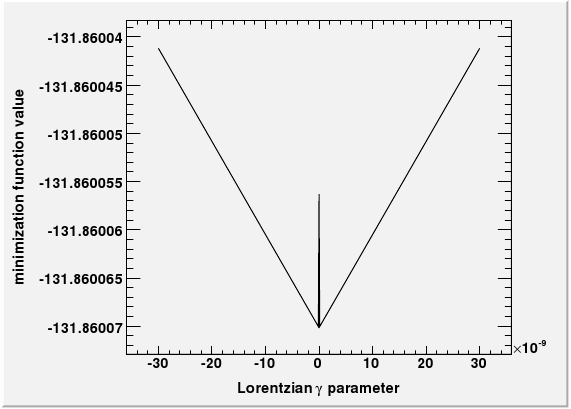
\includegraphics[width=0.4\linewidth]{voigt_gamma.png}

\vspace{-3.4 cm}
\begin{itemize}
\item Old function failed because $\mathcal{L}(\gamma)$ \\ doesn't
  have a parabolic minimum \\ in low-statistics (when $\gamma \ll
  \sigma$)

\item New function:

$\displaystyle f(x) = \left\{ \begin{array}{l l} \exp\left(-\frac{x^2}{2 \sigma^2}\right) & \mbox{if } |x| \le m \\ 1/x^4 & \mbox{if } |x| > m \end{array} \right.$

\item Requiring normalization, continuity, and differentiability sets $m=2\sigma$

\item $1/x^4$ motivated by Rutherford scattering formula
\end{itemize}

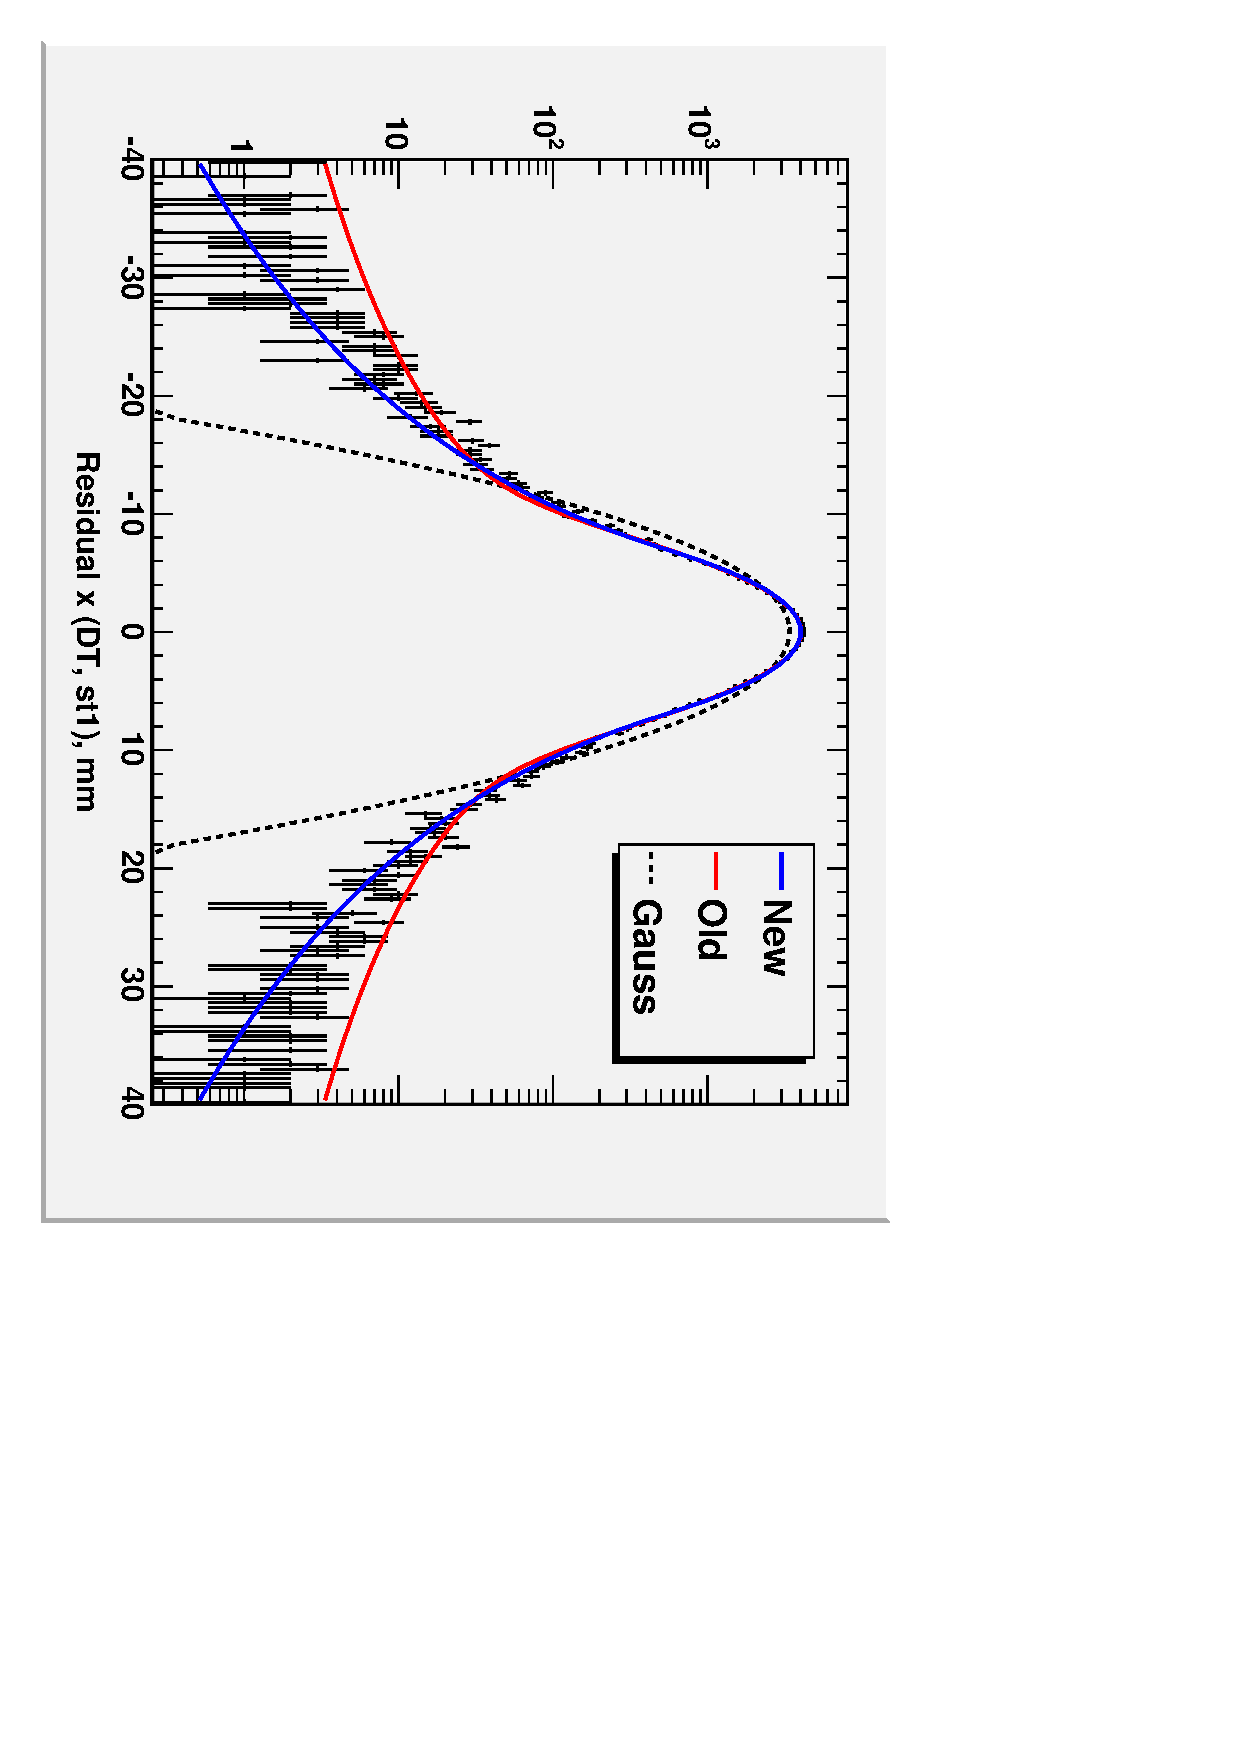
\includegraphics[height=0.49\linewidth, angle=90]{residuals_DT_st2_log.pdf} \hfill
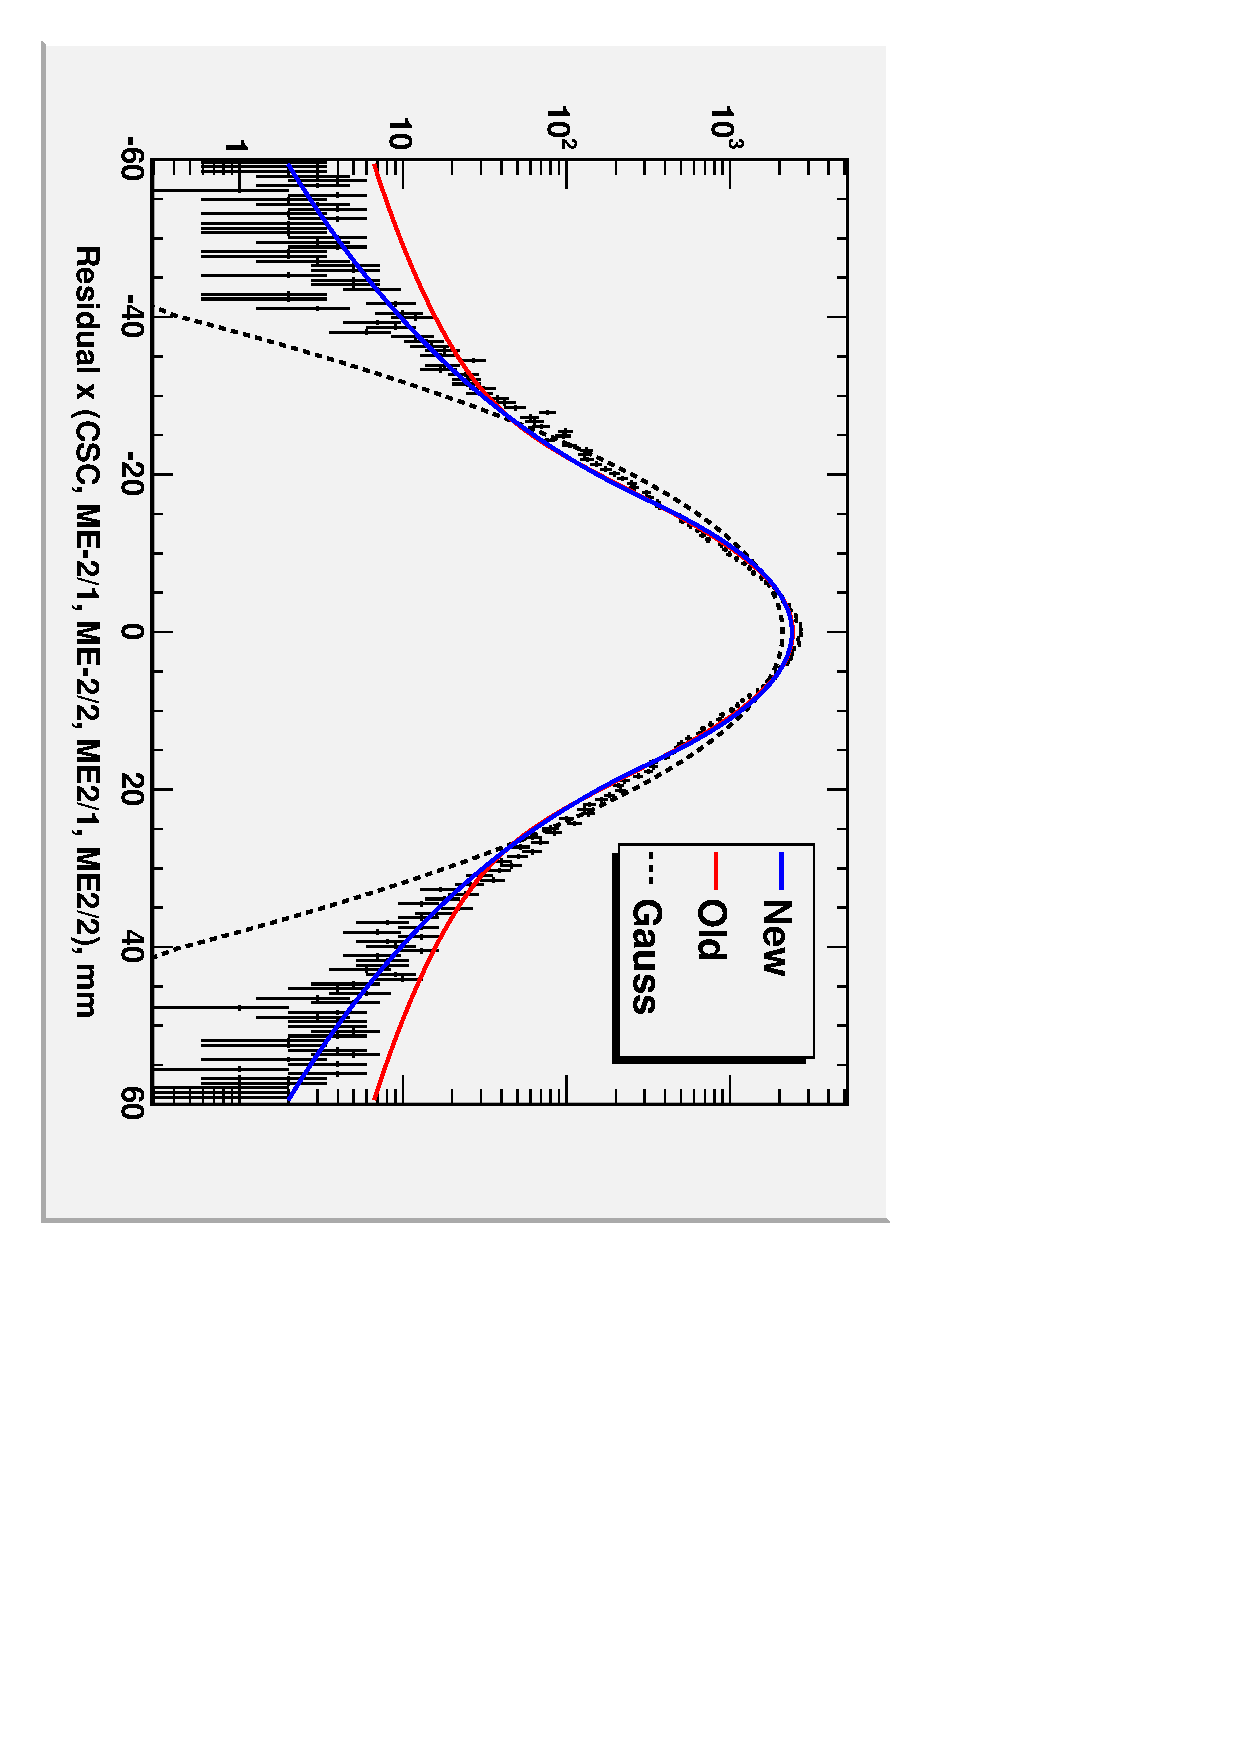
\includegraphics[height=0.49\linewidth, angle=90]{residuals_CSC_21_22_log.pdf}
\end{frame}

\begin{frame}
\frametitle{Validate algorithmic changes}

\begin{itemize}
\item Verify that new algorithm produces the same alignment results as old algorithm for CRAFT-09:

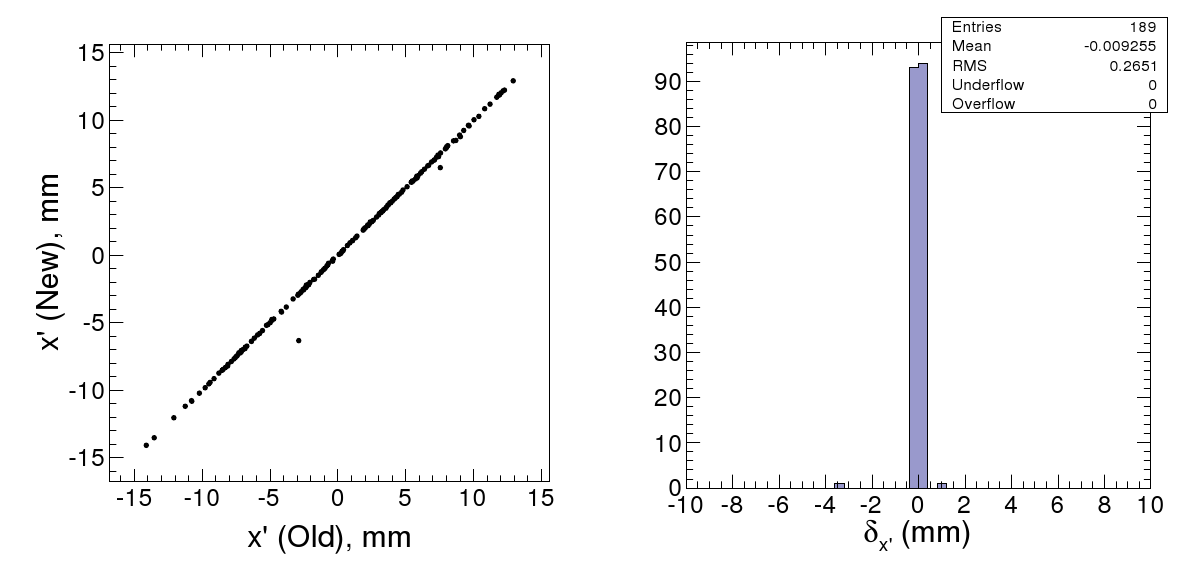
\includegraphics[width=0.95\linewidth]{old-new-validation.png}

\item RMS of 250~$\mu$m differences dominated by two chambers
\begin{itemize}
\item they are low-statistics and did not reach a fixed point in old alignment (values still changing after 5 iterations)
\end{itemize}

\item 189 chambers aligned in old algorithm, compared above

\item all 250 chambers aligned in new algorithm
\end{itemize}
\end{frame}

\begin{frame}
\frametitle{Comparison of 2009 with 2010}

\begin{itemize}
\item Did chambers physically move during the winter shut-down?

\item Plot CRAFT-09, CRAFT-10 differences
\end{itemize}

\begin{center}
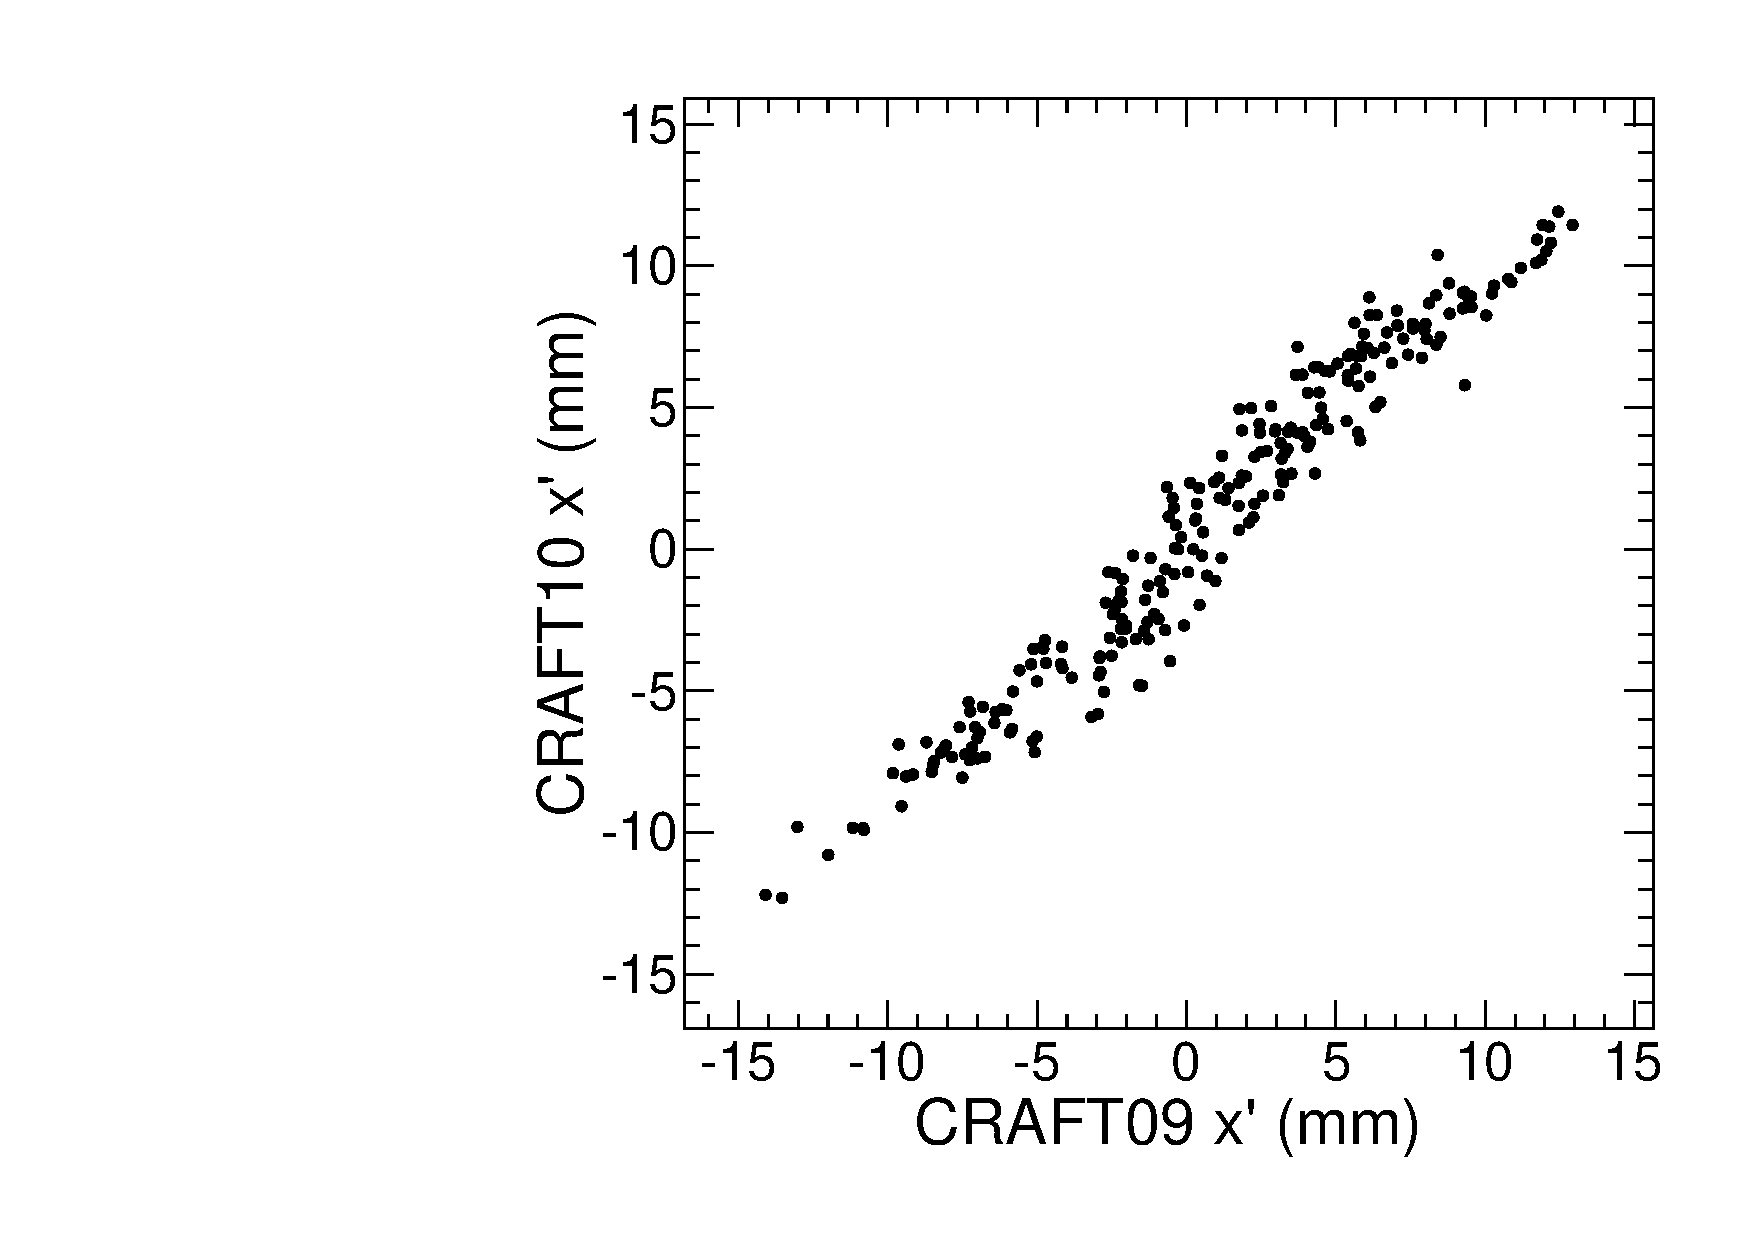
\includegraphics[width=0.3\linewidth]{craft09_craft10_x_corr.pdf}
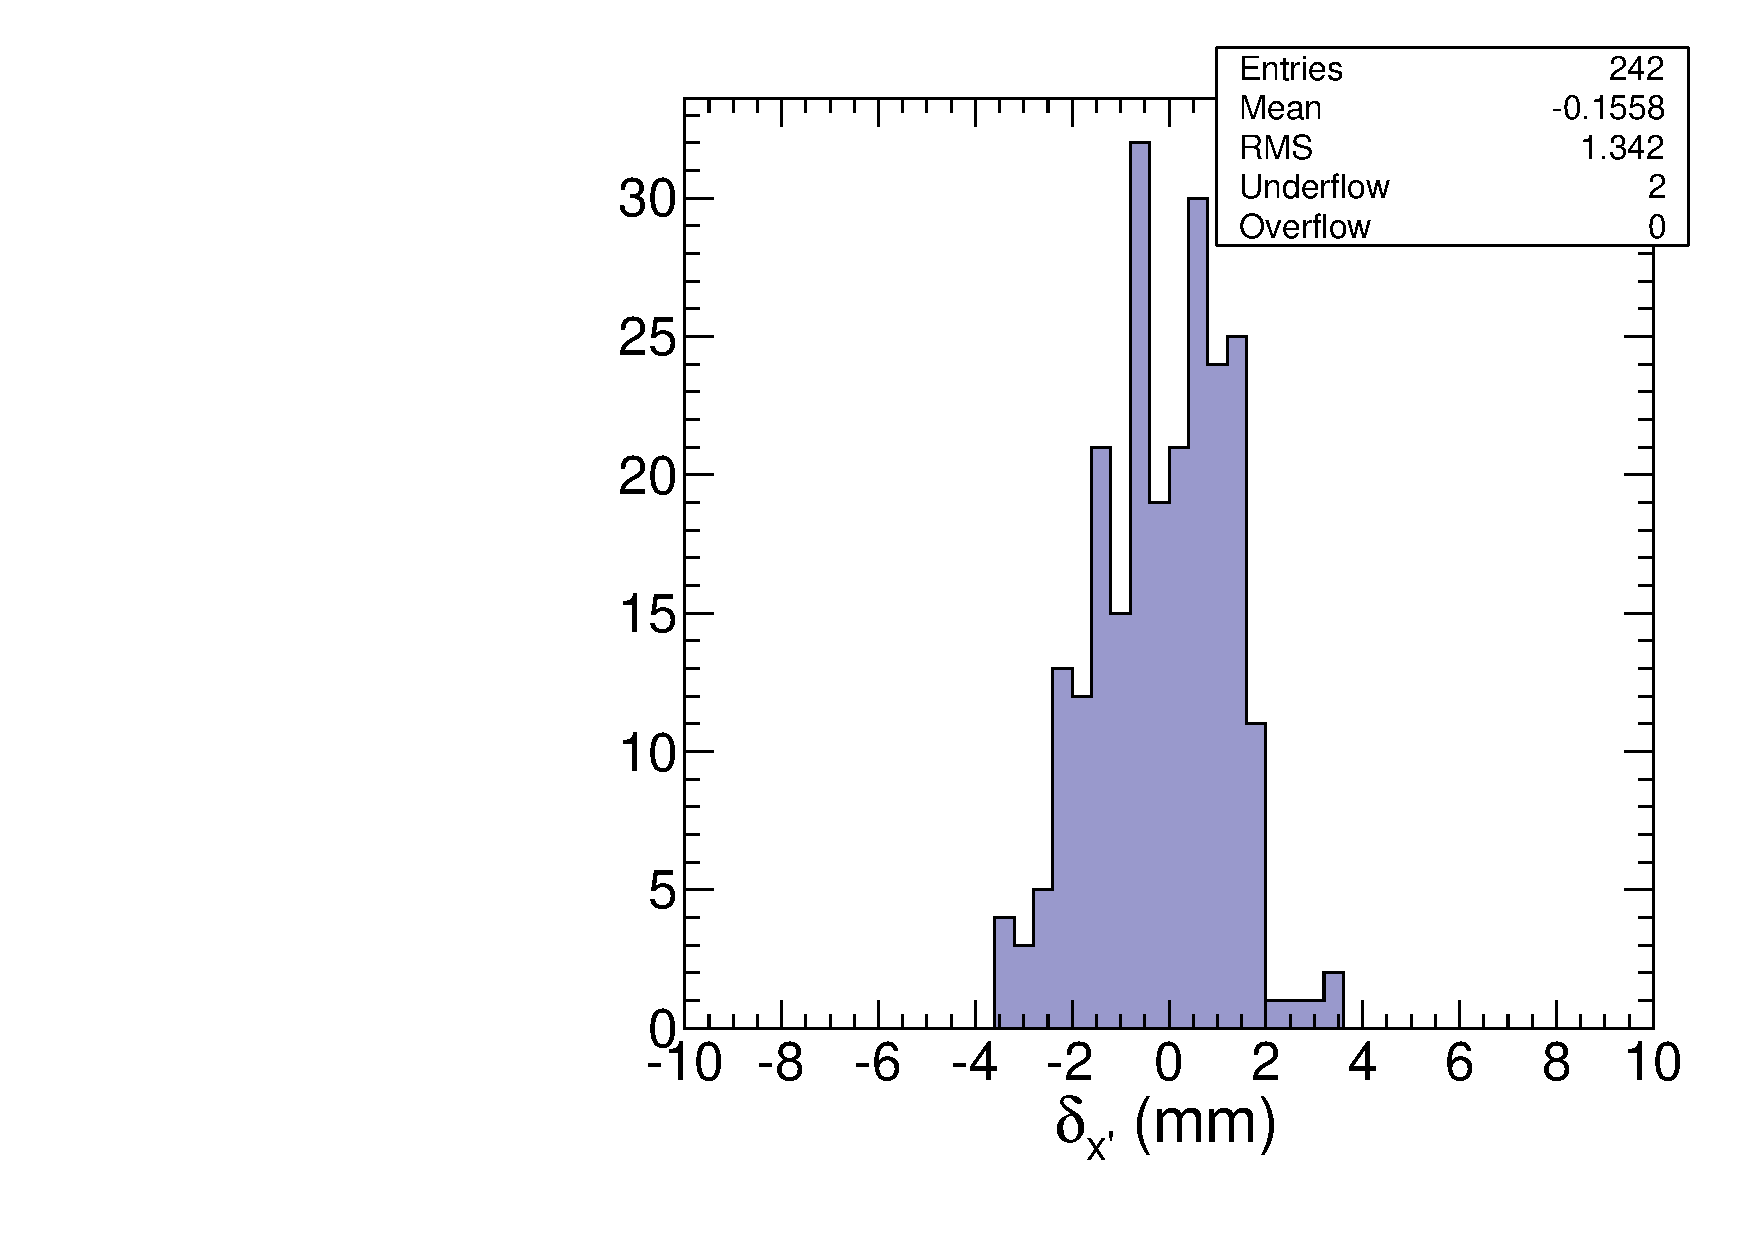
\includegraphics[width=0.3\linewidth]{craft09_craft10_x_diff.pdf} \hspace{1 cm}

\hspace{1 cm} 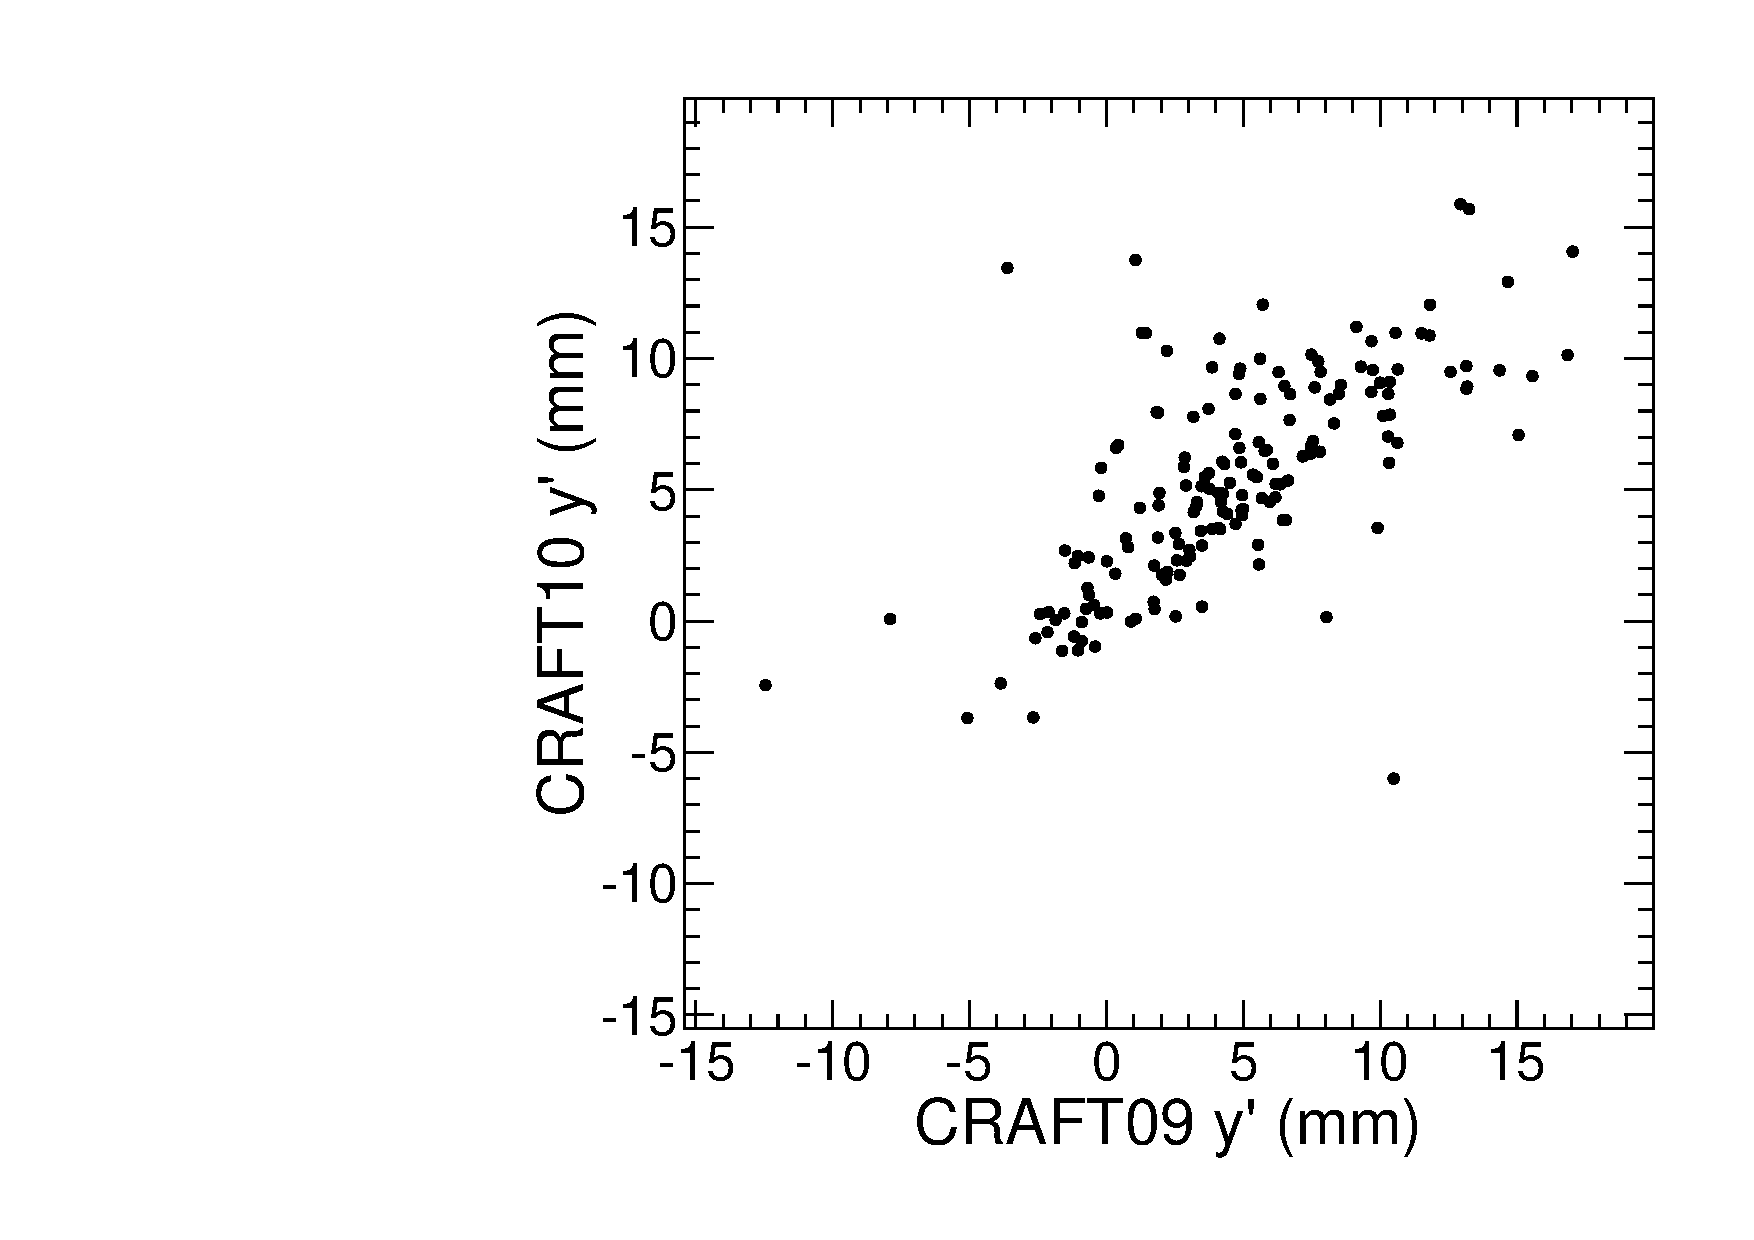
\includegraphics[width=0.3\linewidth]{craft09_craft10_y_corr.pdf}
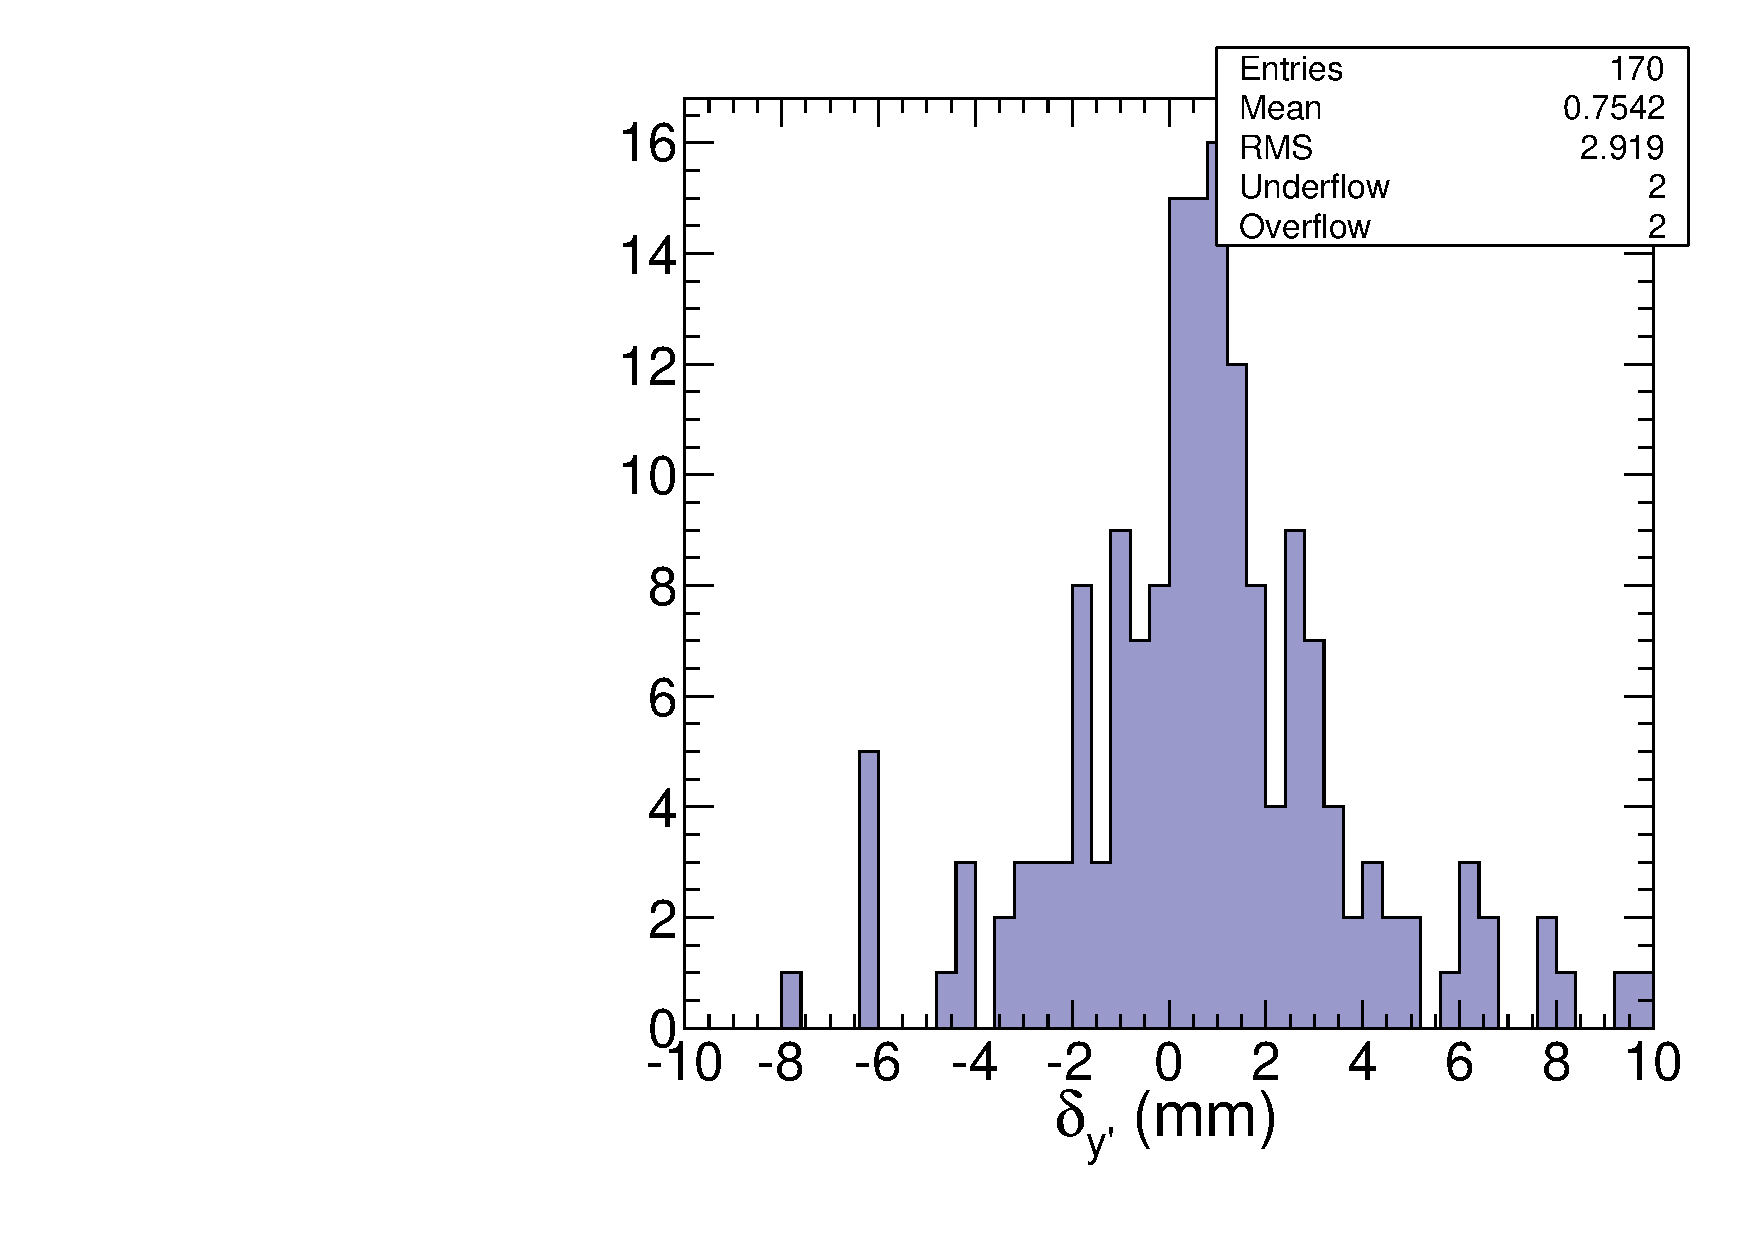
\includegraphics[width=0.3\linewidth]{craft09_craft10_y_diff.pdf}
\end{center}
\end{frame}

\begin{frame}
\frametitle{Comparison of 2009 with 2010}

\begin{itemize}
\item Is there a pattern in these differences?  Yes!

\begin{columns}
\column{0.05\linewidth}
\column{0.4\linewidth}
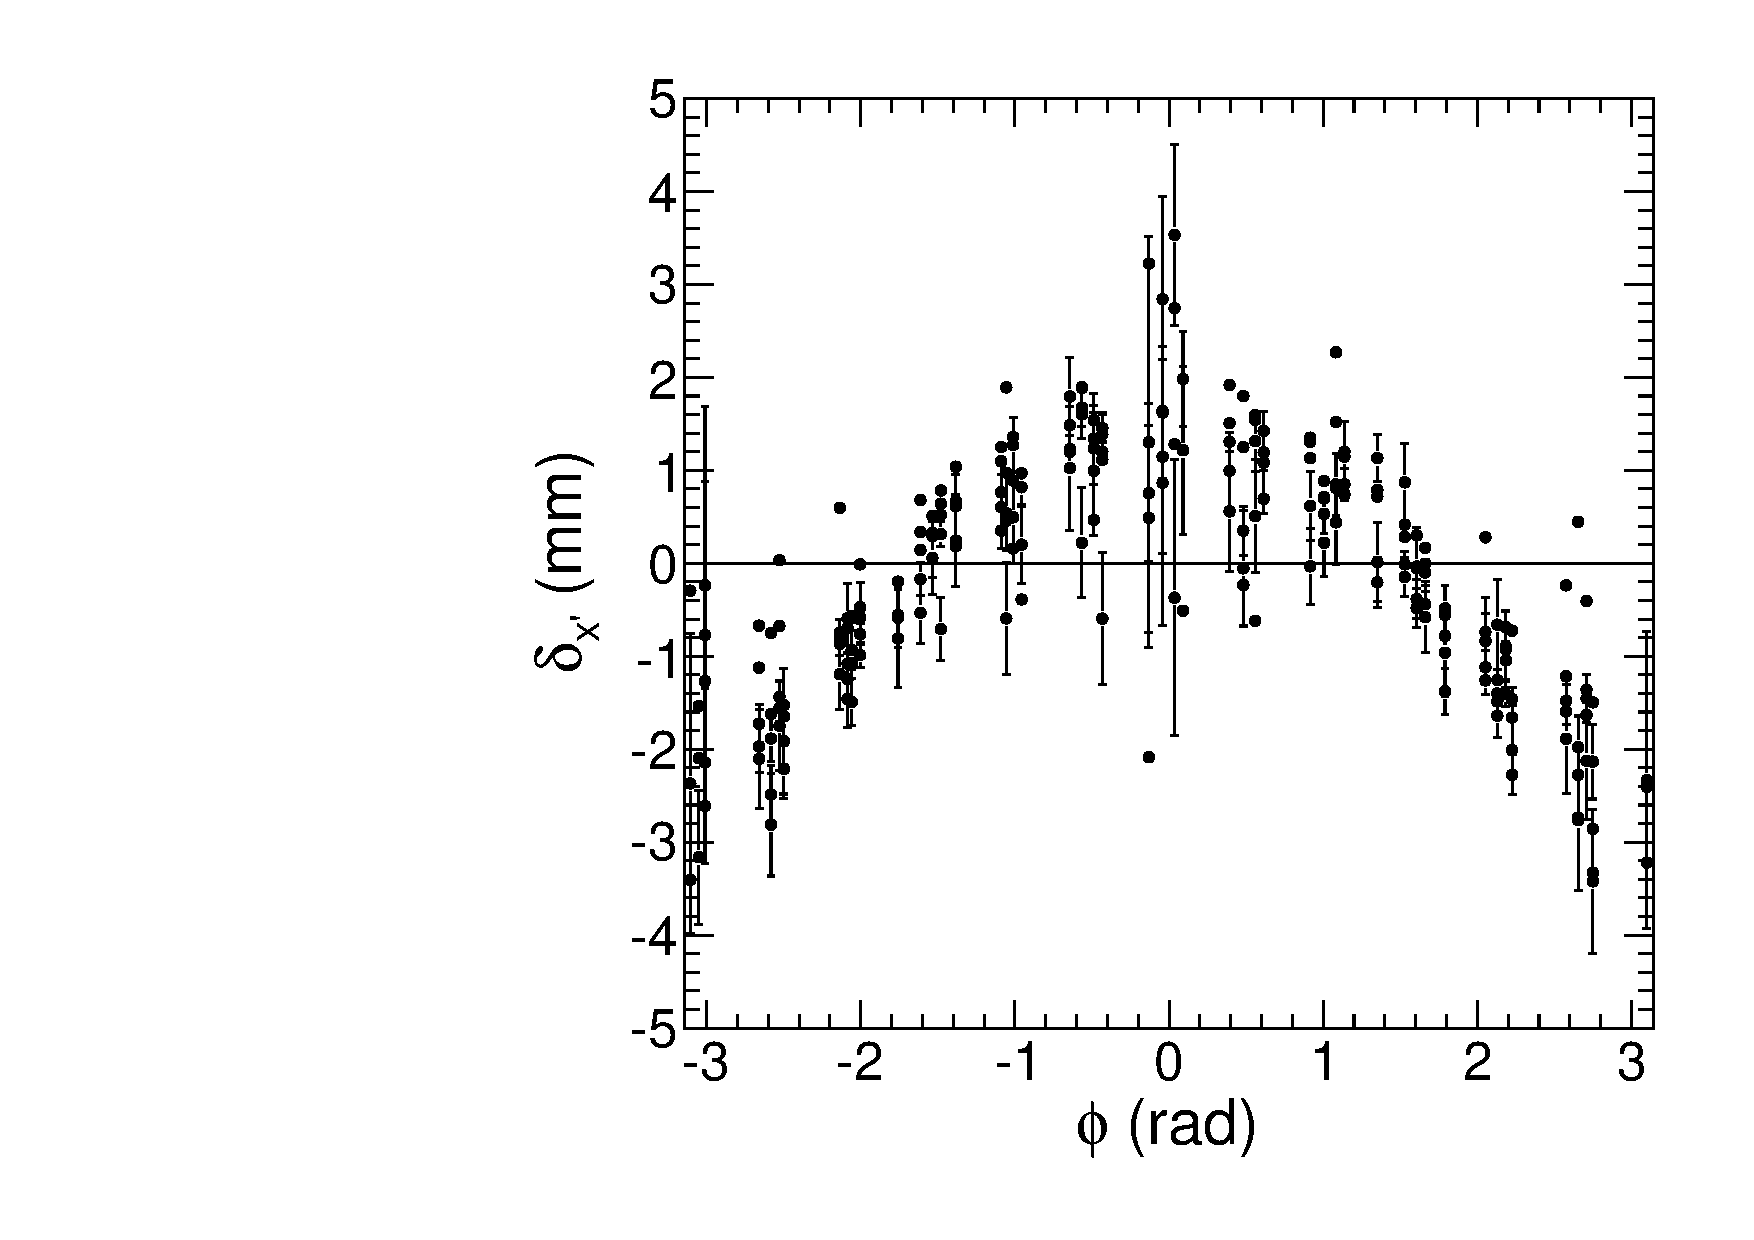
\includegraphics[width=\linewidth]{craft09_craft10_x_phi.pdf}
\column{0.05\linewidth}
\hfill {\bf $\longrightarrow$} \hfill
\column{0.4\linewidth}
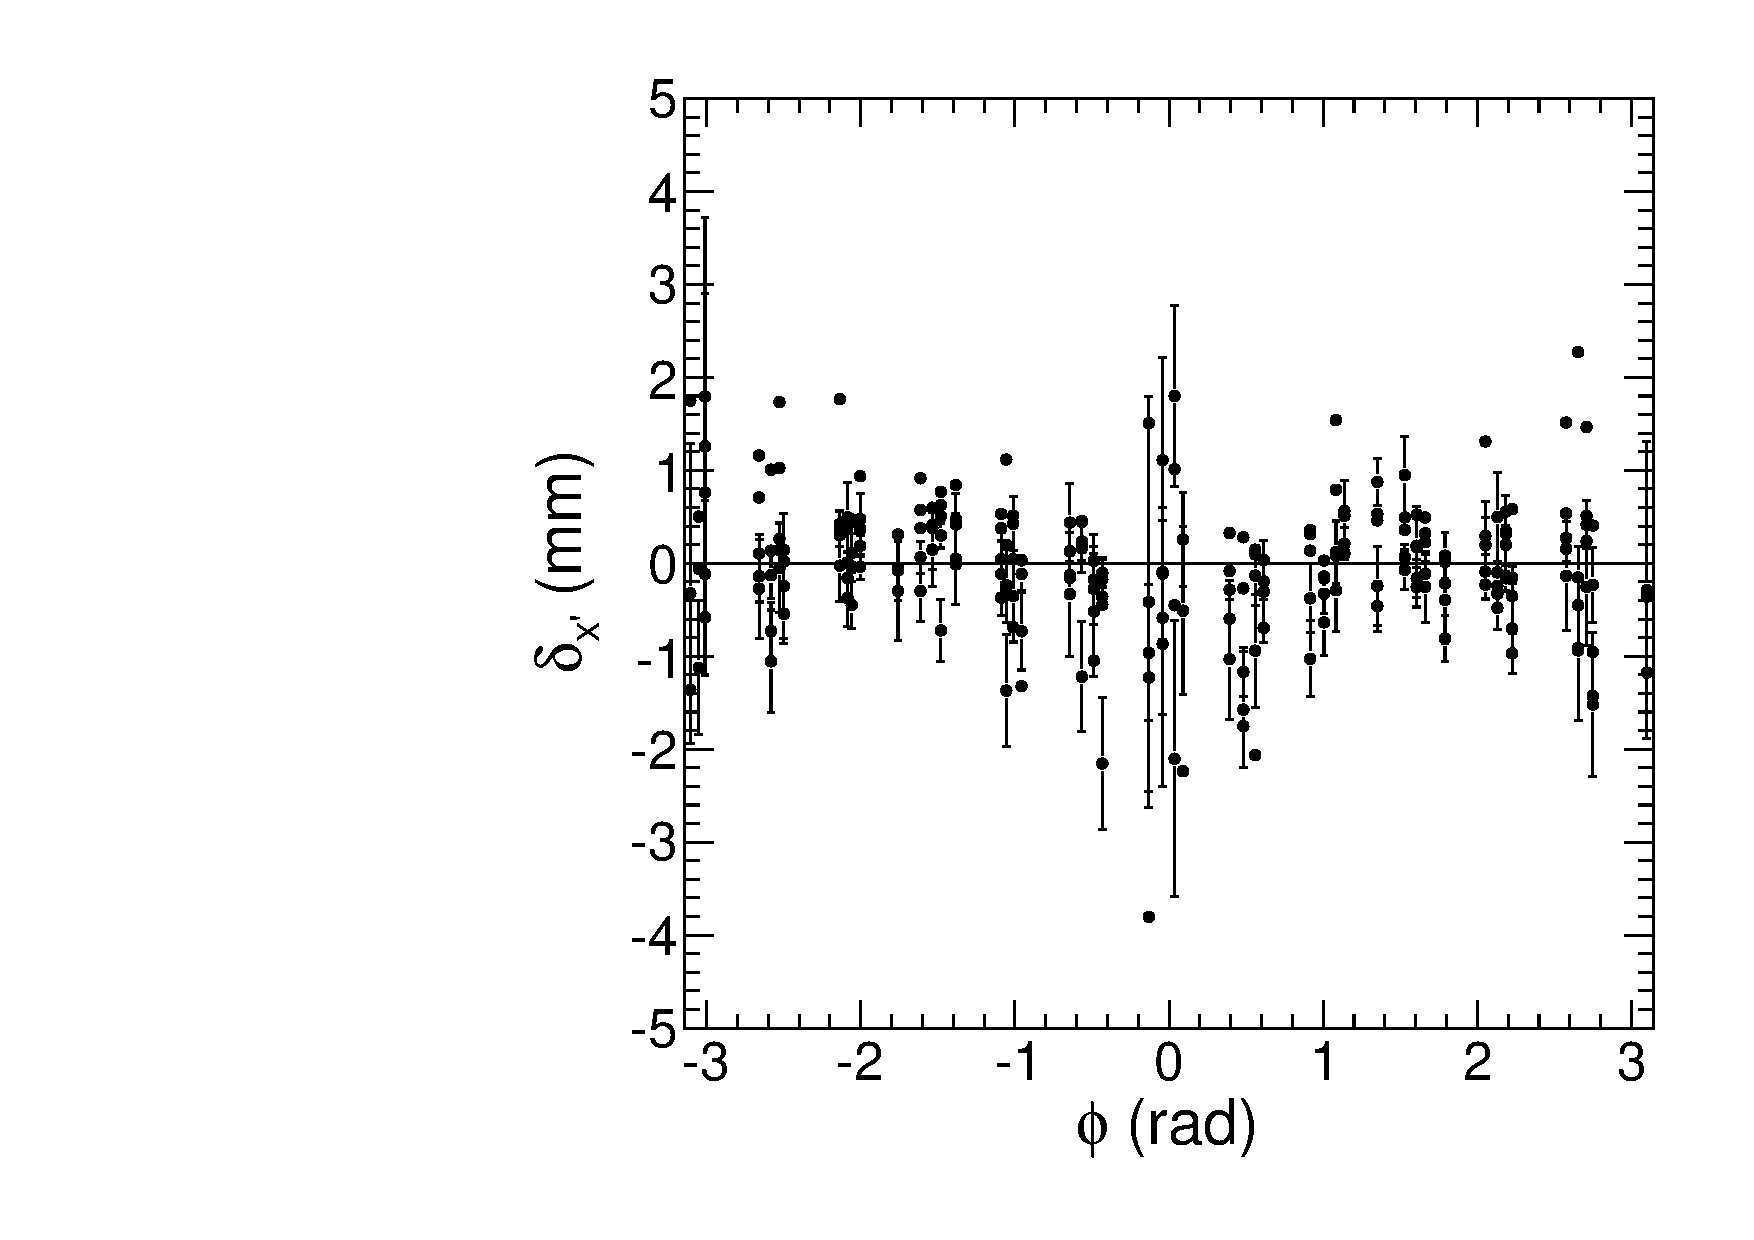
\includegraphics[width=\linewidth]{craft09_craft10_x_phi_real.pdf}
\column{0.05\linewidth}
\end{columns}

\item Most of the variation is in a $\sin\phi + \cos\phi + \mbox{const}$ trend (mostly $\cos$)

\item These bulk trends only reflect changes in global position (possibly a GlobalPositionRcd issue)

\item Subtract out this trend so that we can analyze only internal alignment of the muon system
\end{itemize}
\end{frame}

\begin{frame}
\frametitle{Comparison of 2009 with 2010}

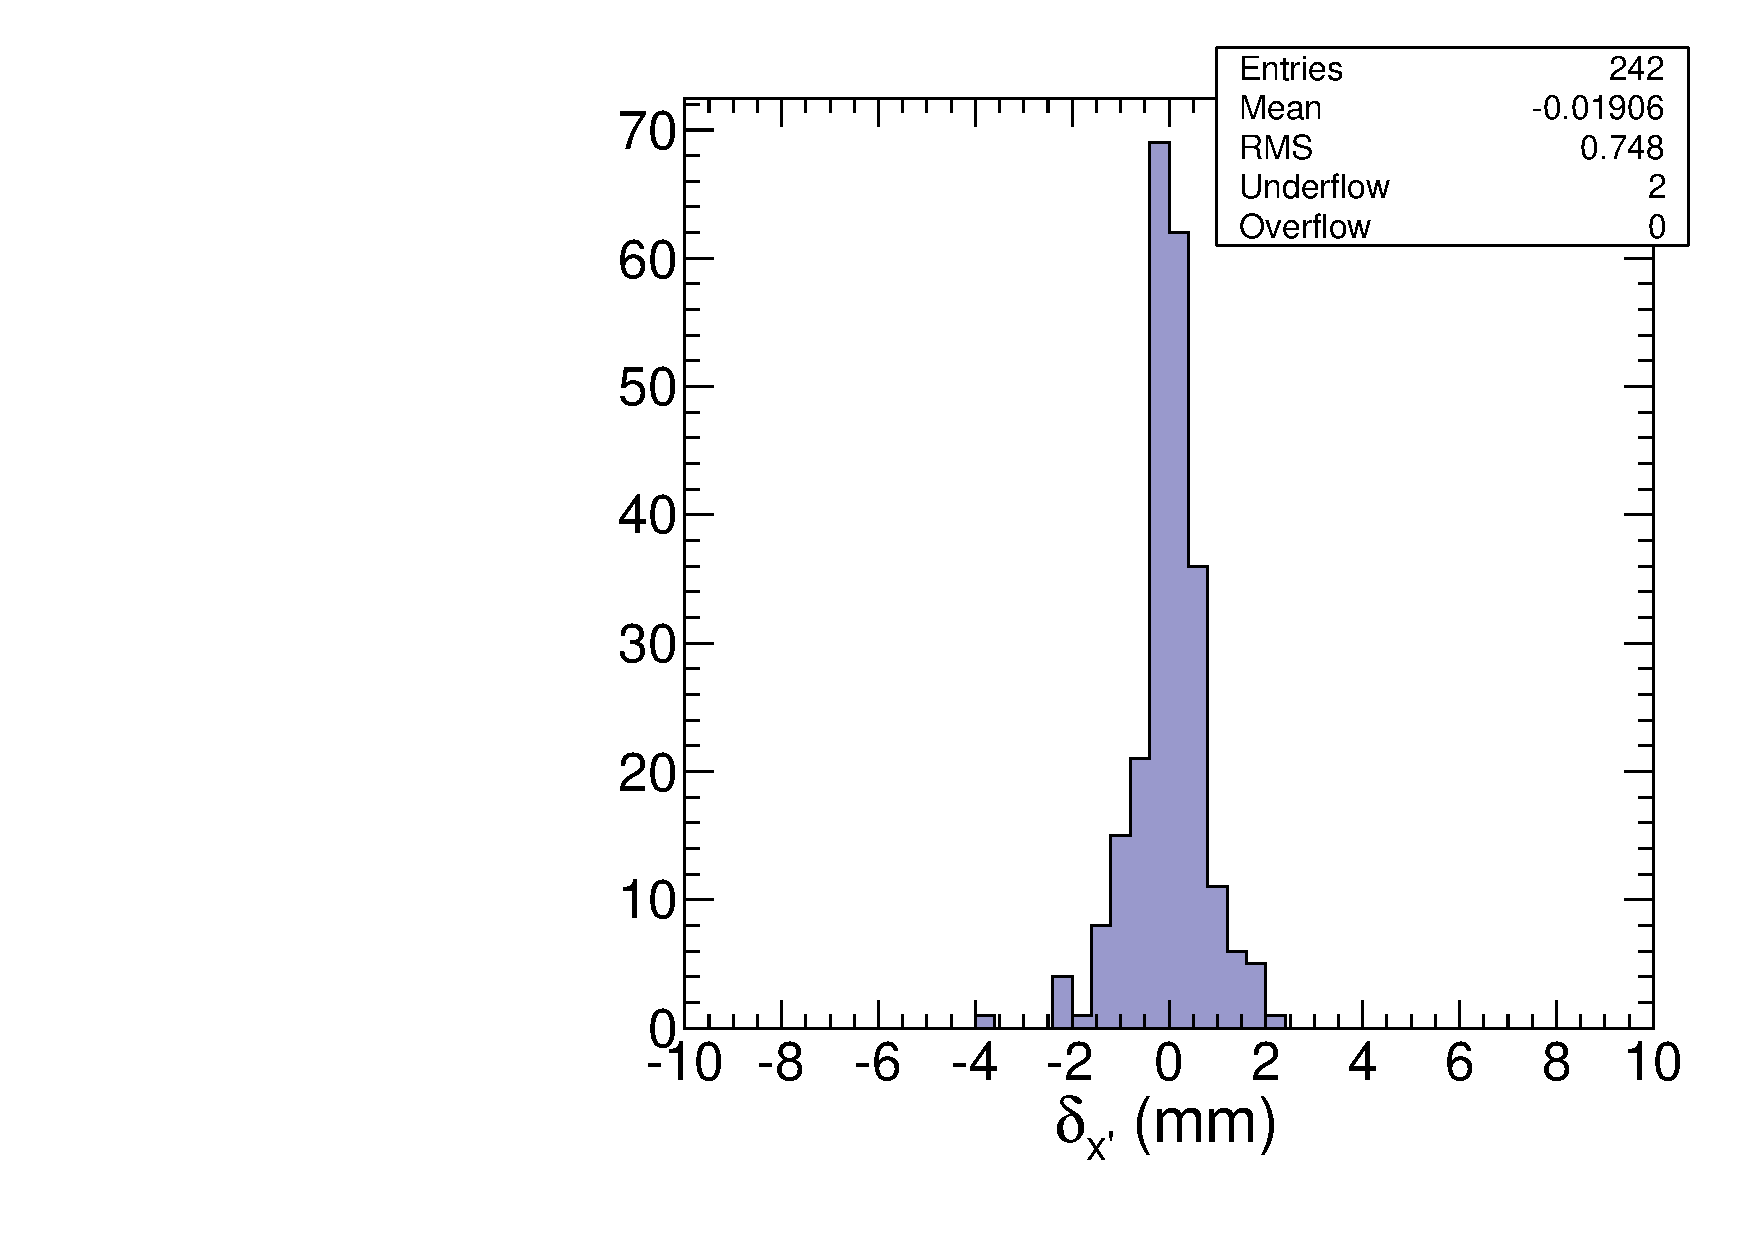
\includegraphics[width=0.5\linewidth]{craft09_craft10_x_realdiff.pdf} \hfill
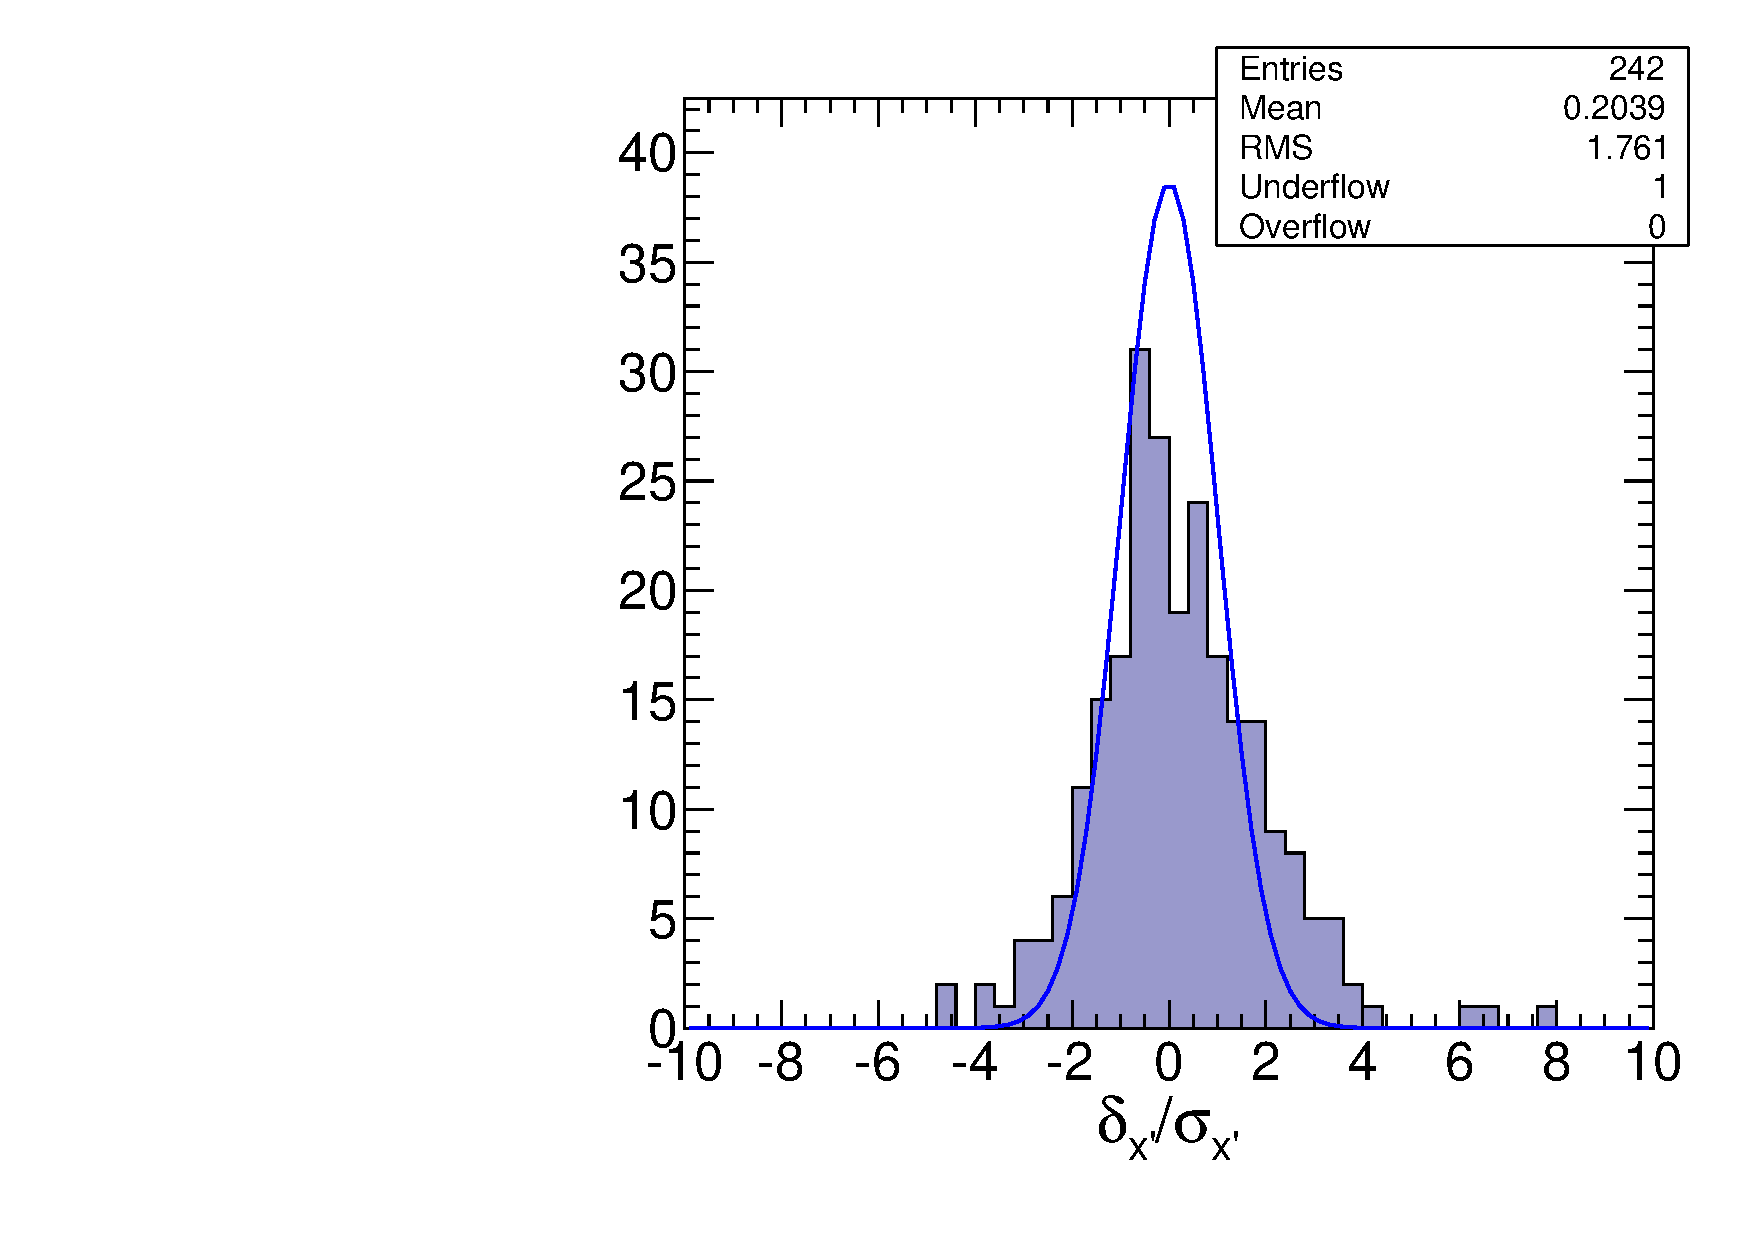
\includegraphics[width=0.5\linewidth]{craft09_craft10_x_realdiff_norm.pdf}

\begin{itemize}
\item Random variations around the $\cos\phi$ curve are 0.75~mm wide and almost pure statistics
\end{itemize}
\end{frame}

\begin{frame}
\frametitle{2010 hardware alignment}

\begin{itemize}
\item How do hardware and track-based alignments compare in 2010?  Use same method of comparison (also dominated by $\cos\phi$)
\end{itemize}

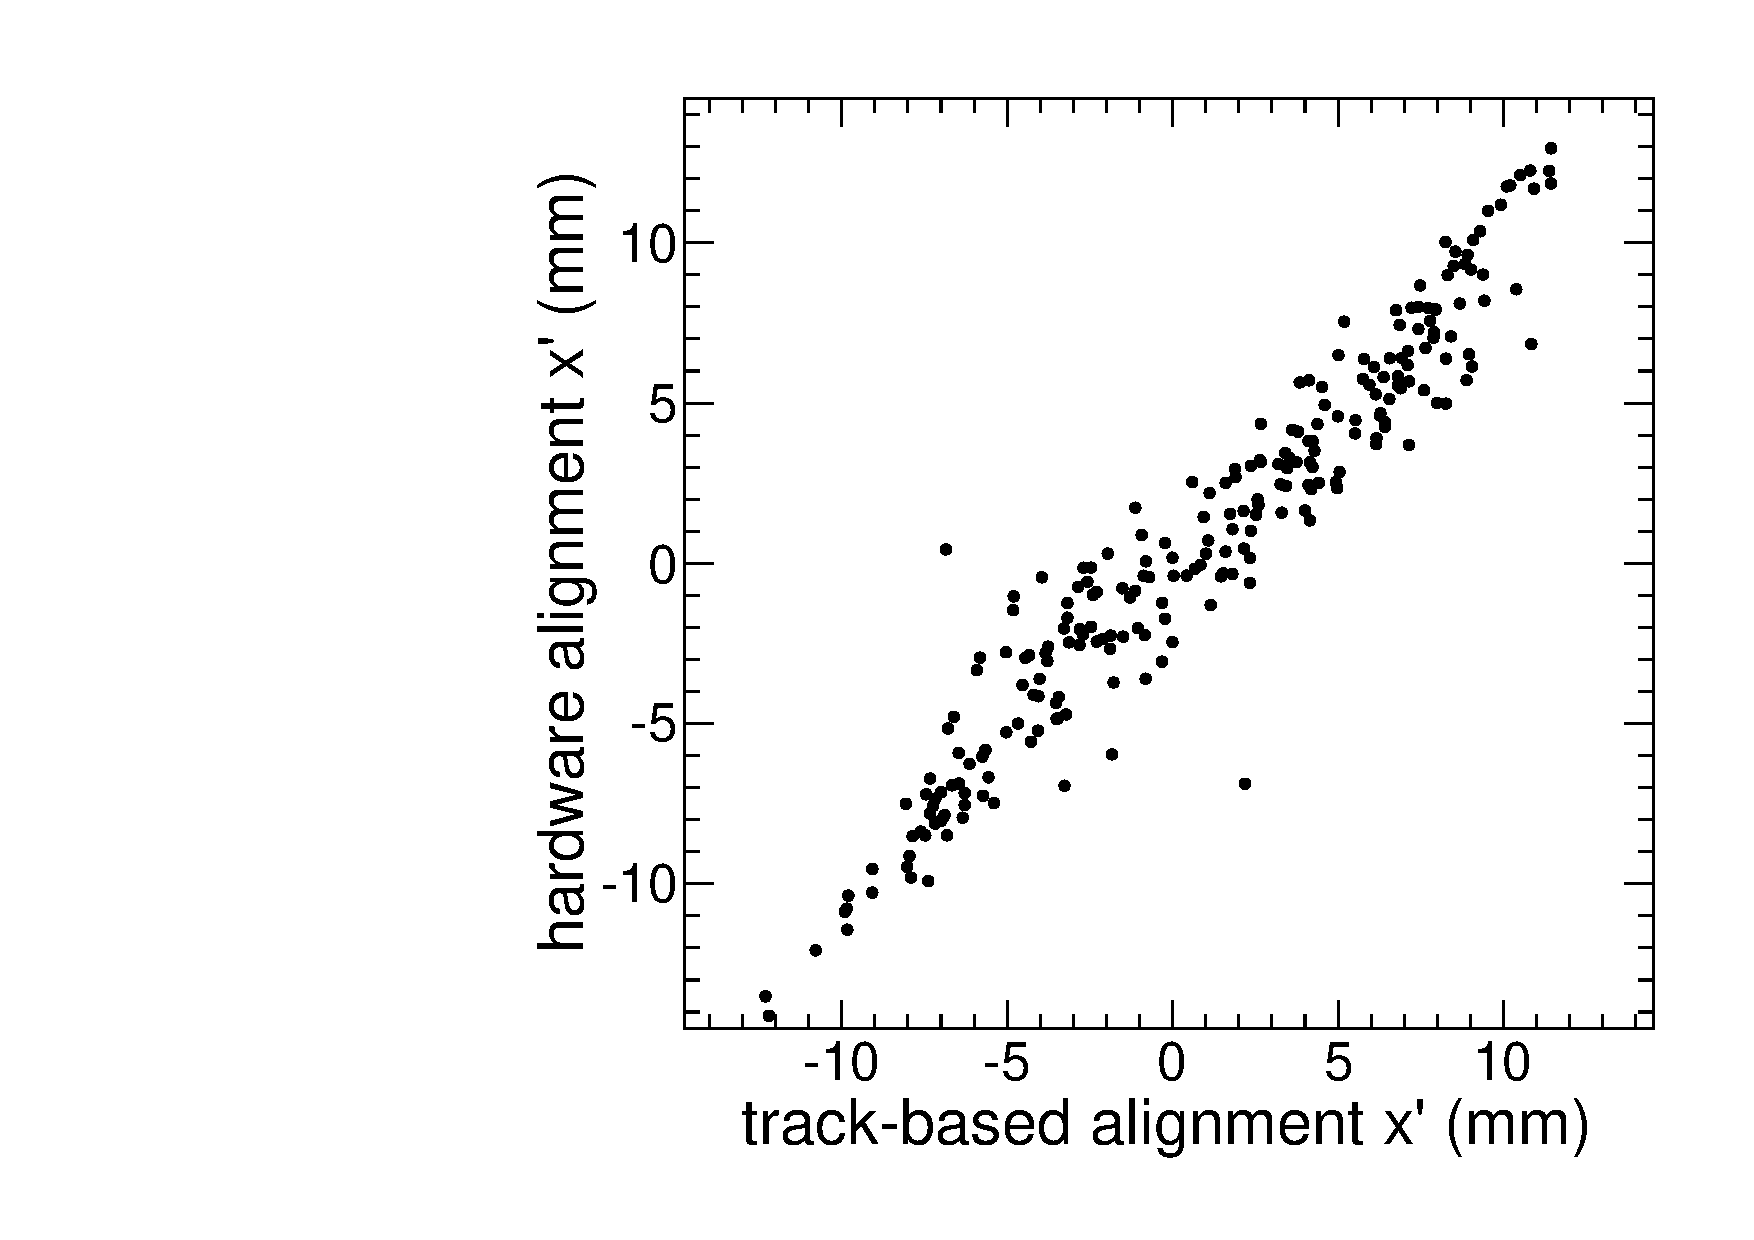
\includegraphics[width=0.33\linewidth]{hardware_x_corr.pdf}
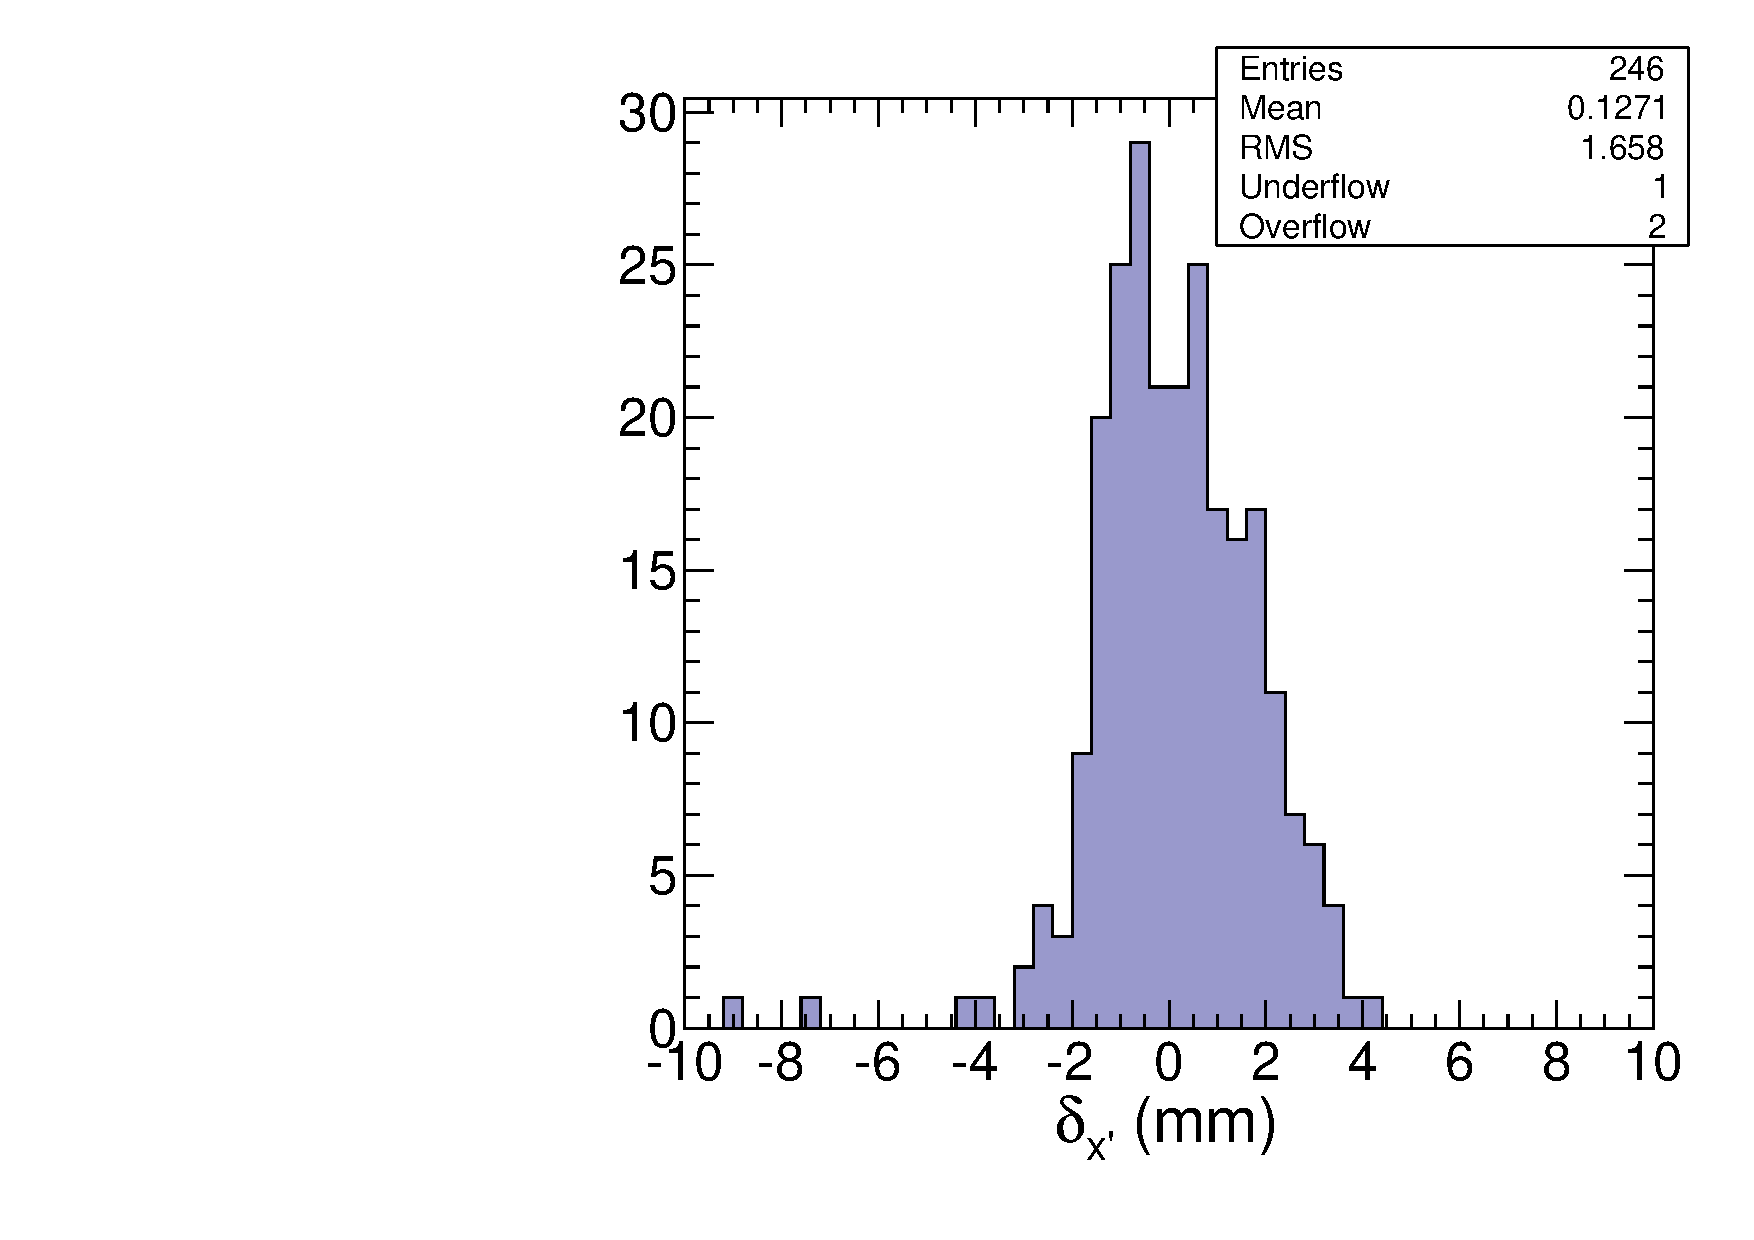
\includegraphics[width=0.33\linewidth]{hardware_x_diff.pdf}
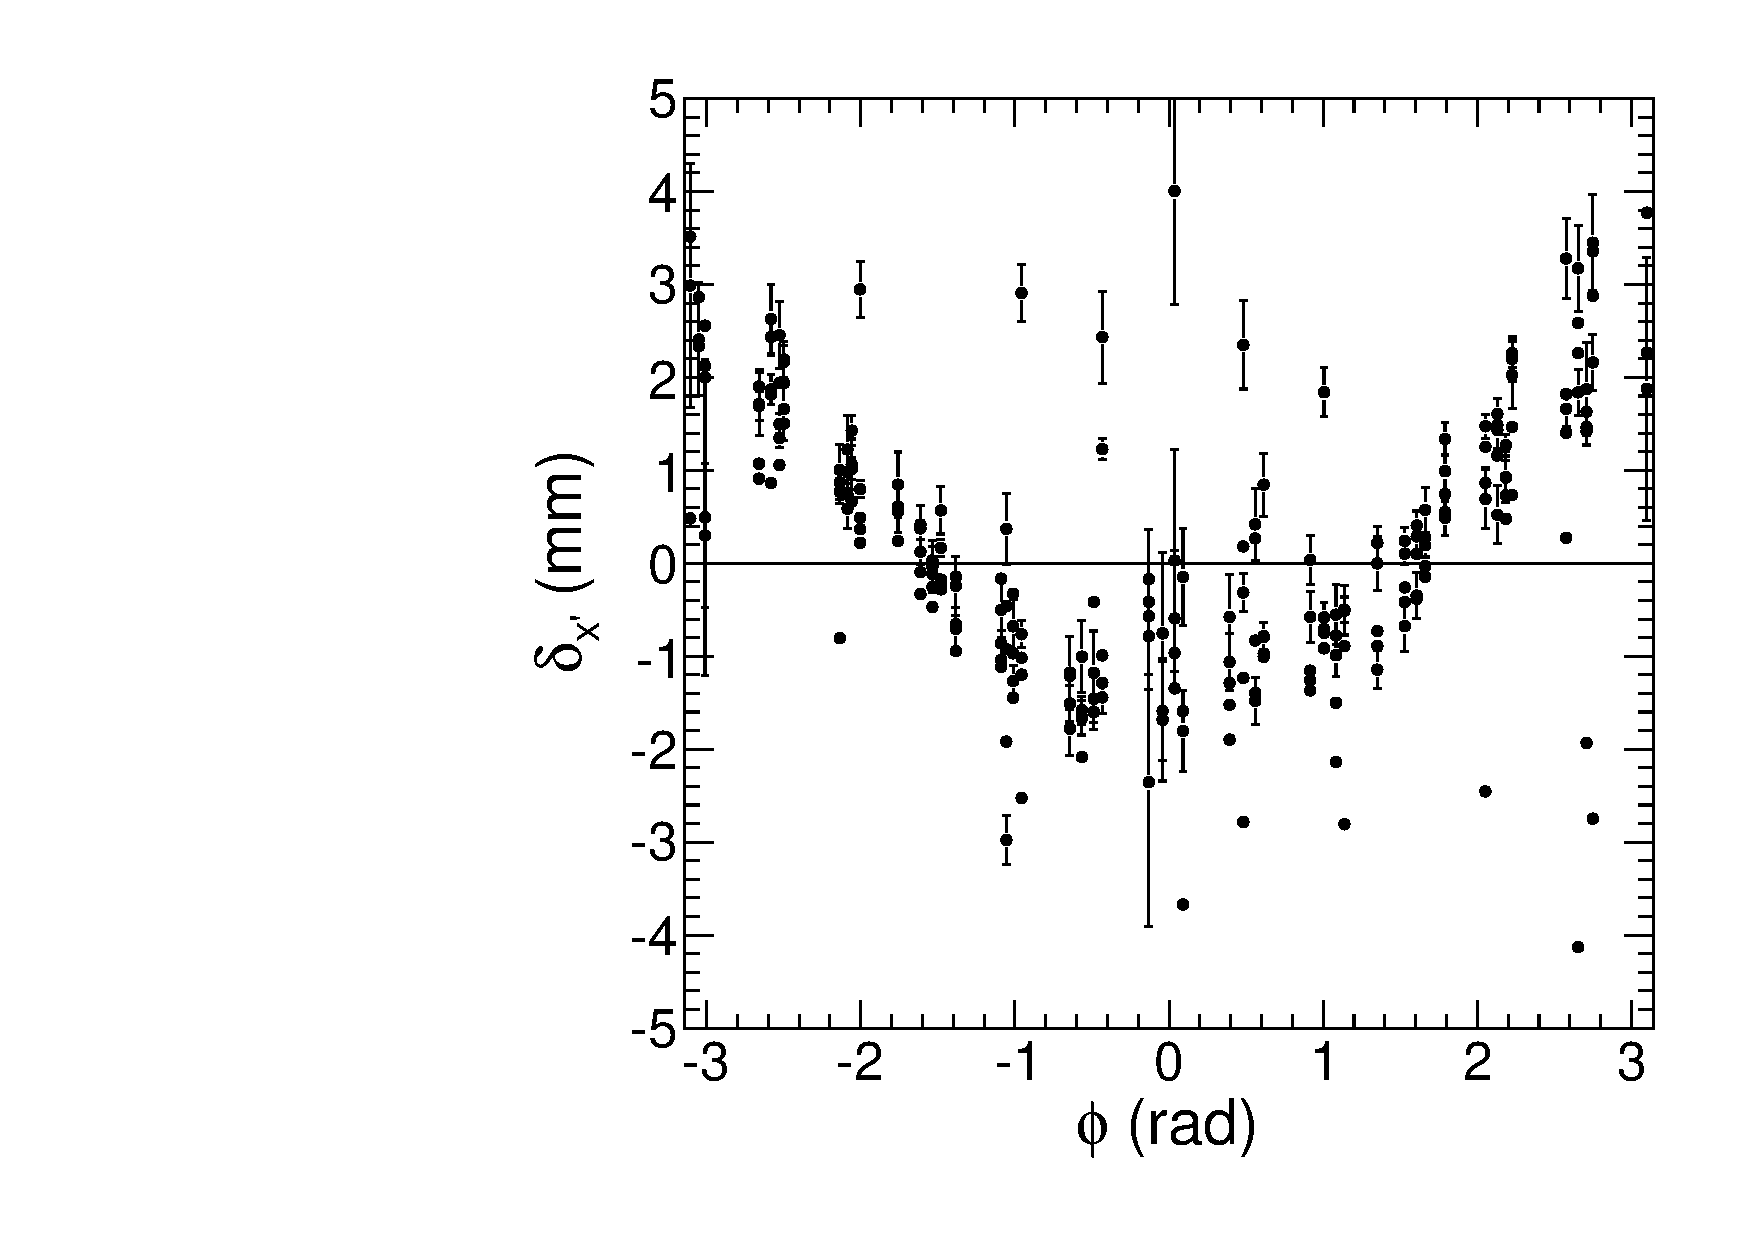
\includegraphics[width=0.33\linewidth]{hardware_x_phi.pdf}

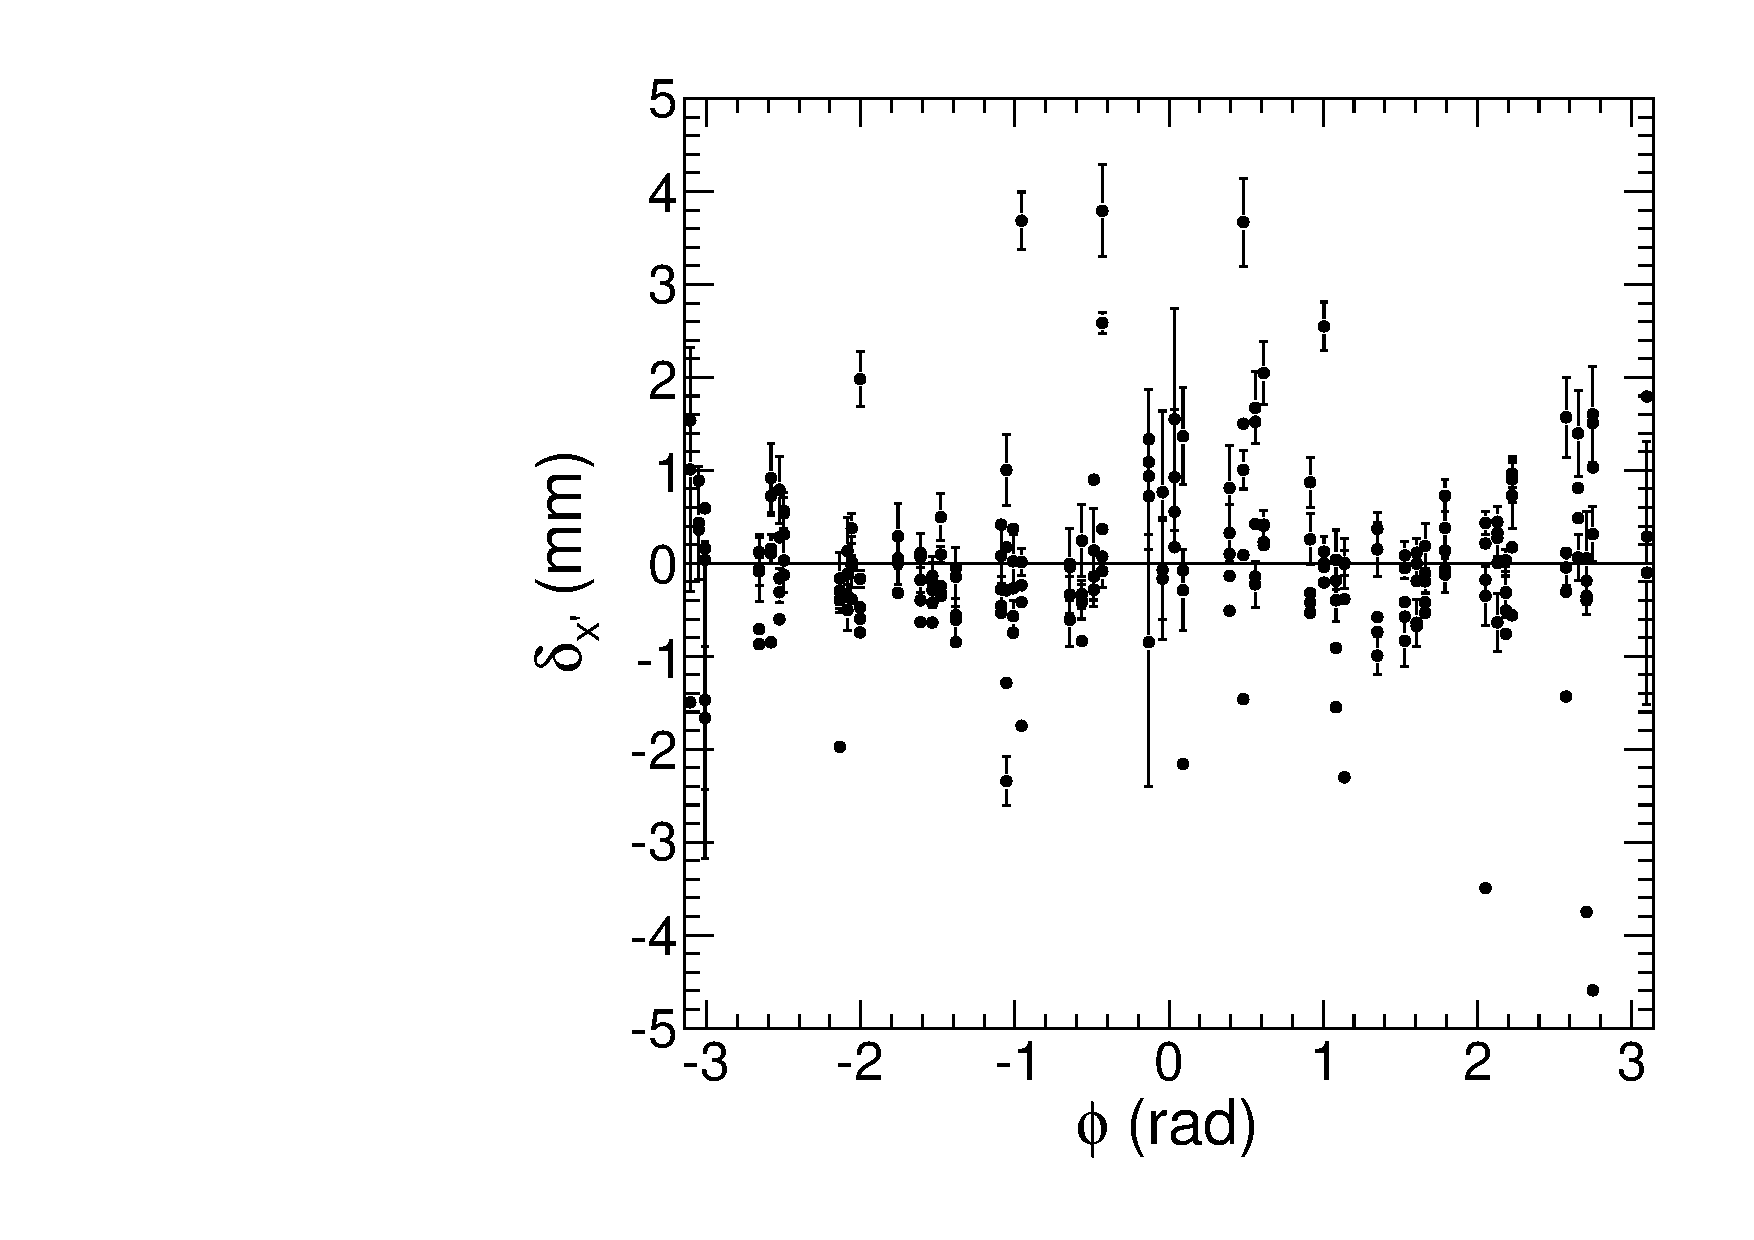
\includegraphics[width=0.33\linewidth]{hardware_x_phi_real.pdf}
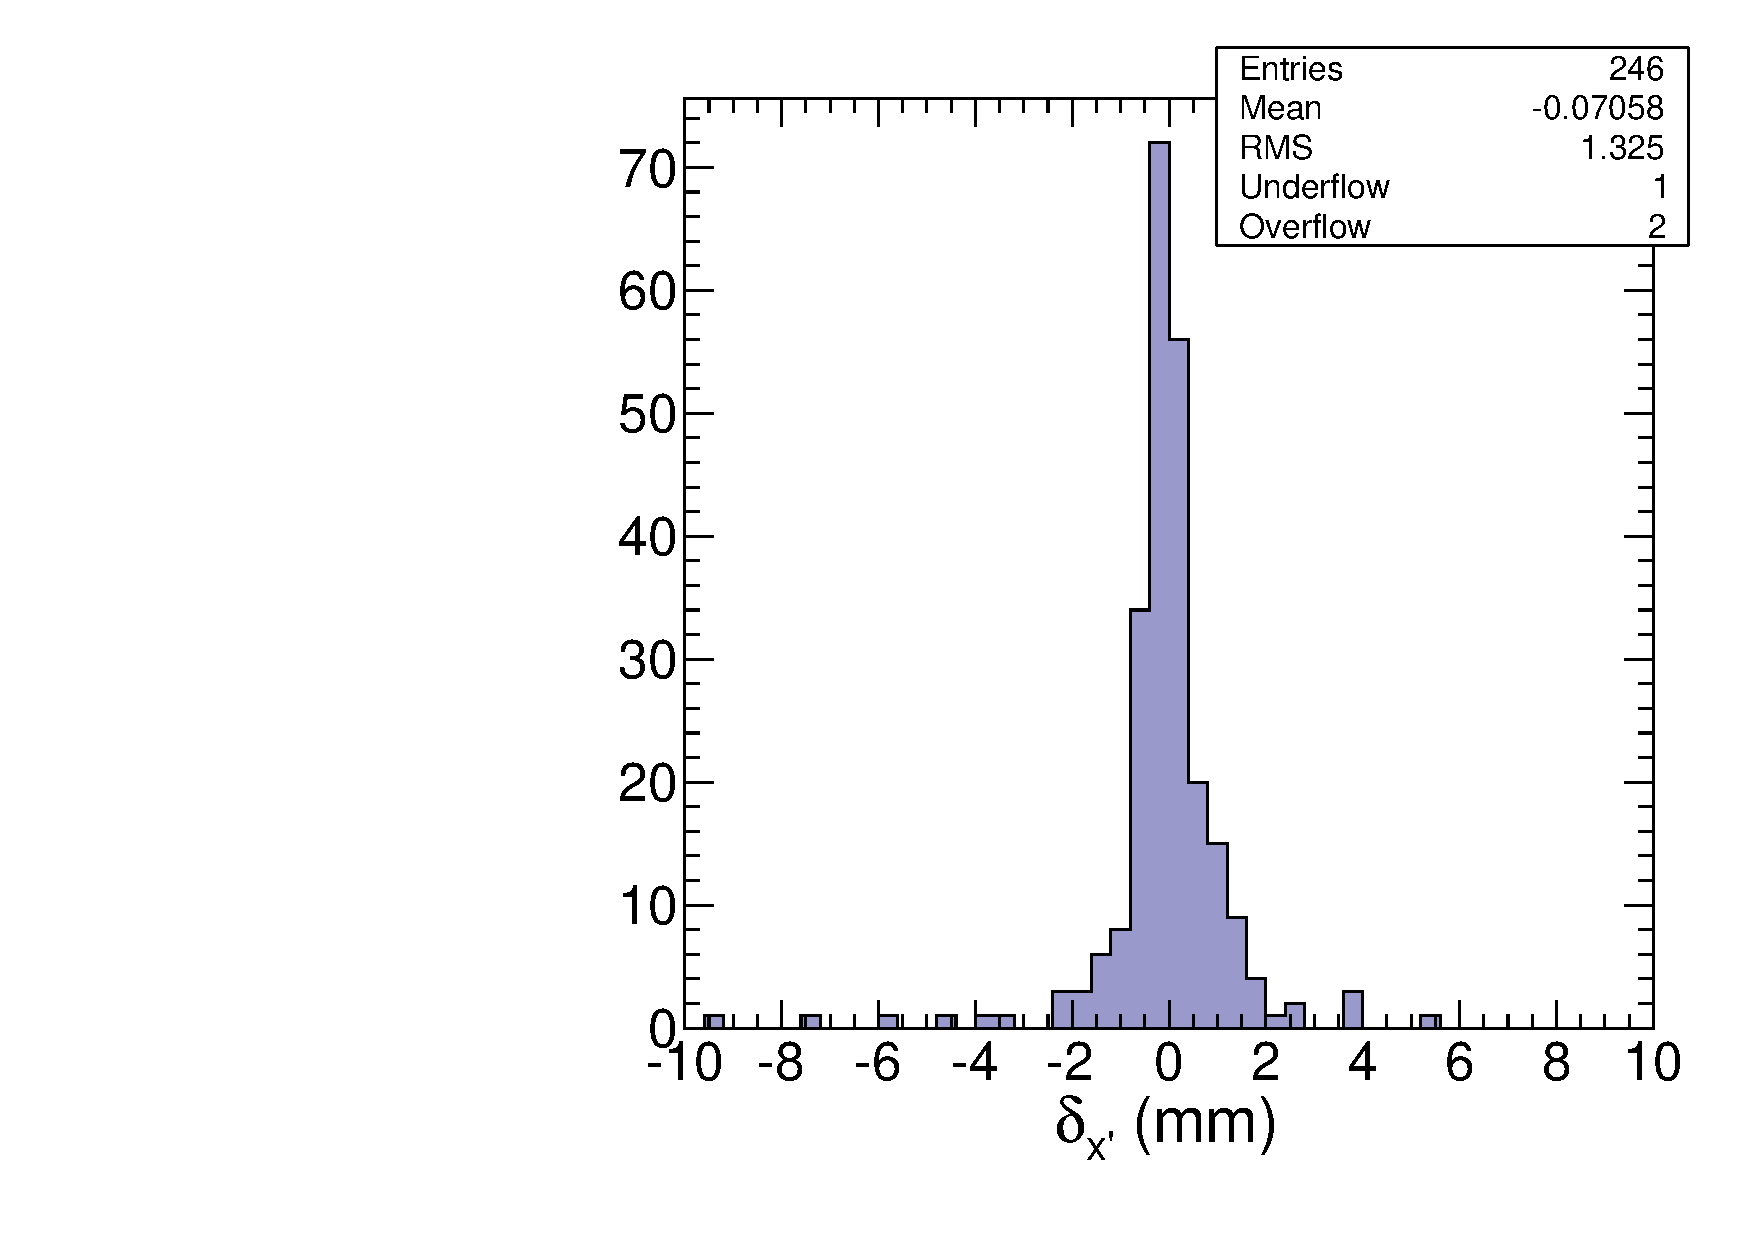
\includegraphics[width=0.33\linewidth]{hardware_x_realdiff.pdf}
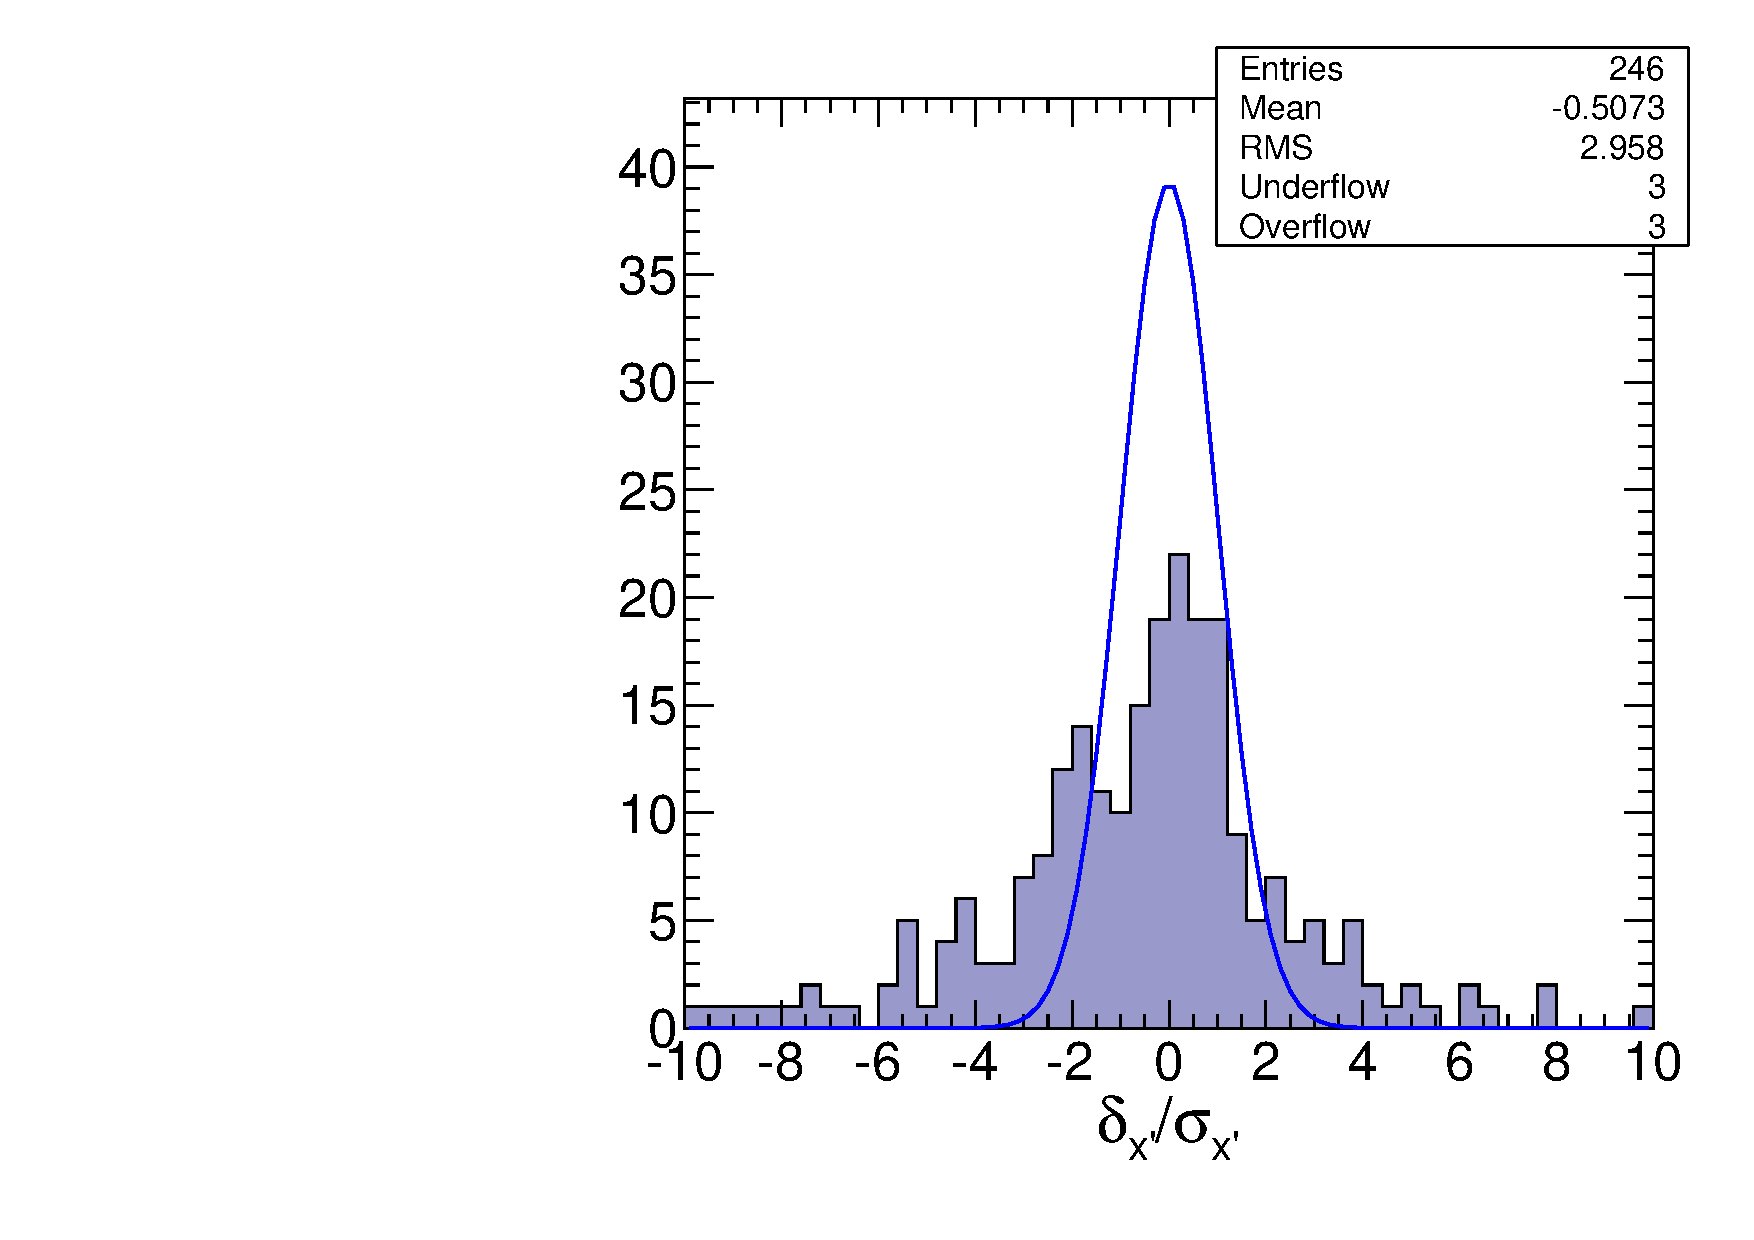
\includegraphics[width=0.33\linewidth]{hardware_x_realdiff_norm.pdf}
\end{frame}

\begin{frame}
\frametitle{2010 hardware alignment}

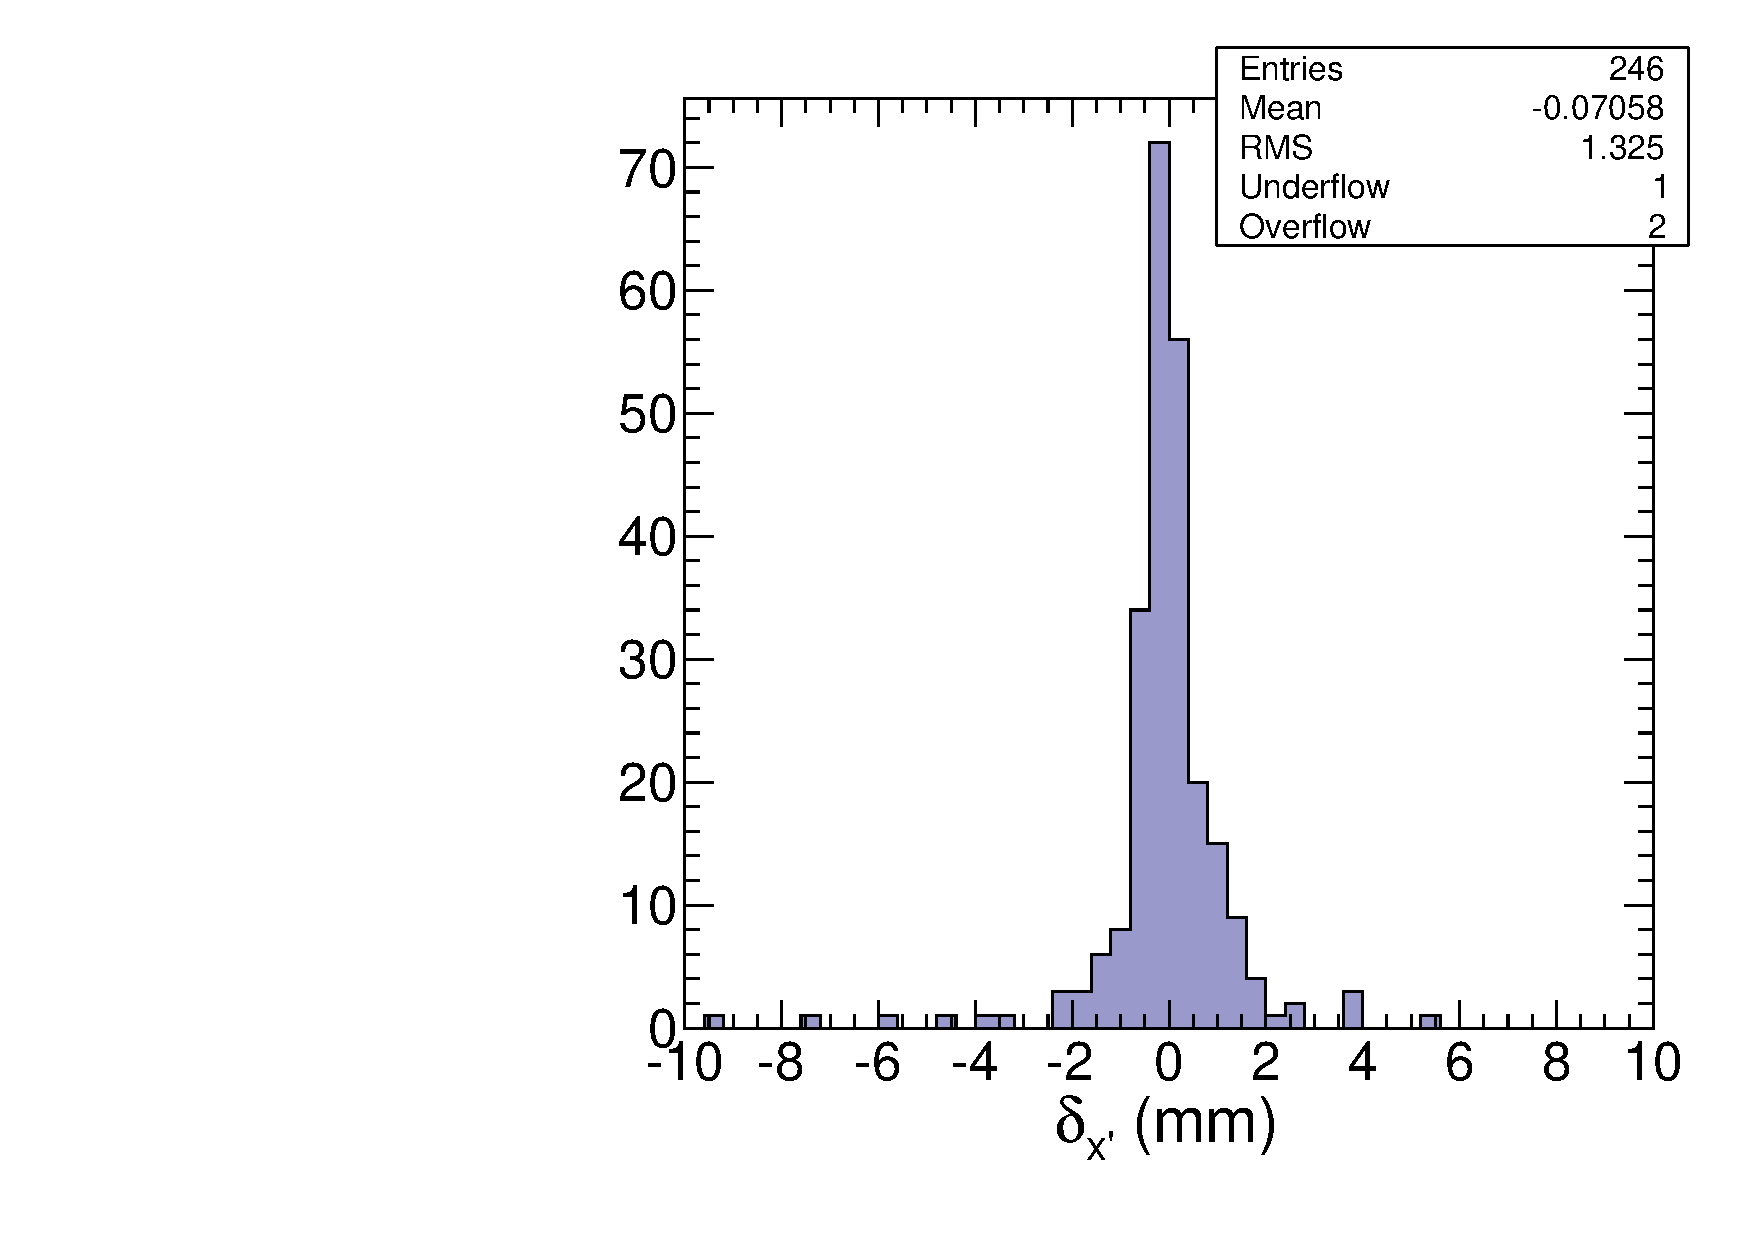
\includegraphics[width=0.33\linewidth]{hardware_x_realdiff.pdf}
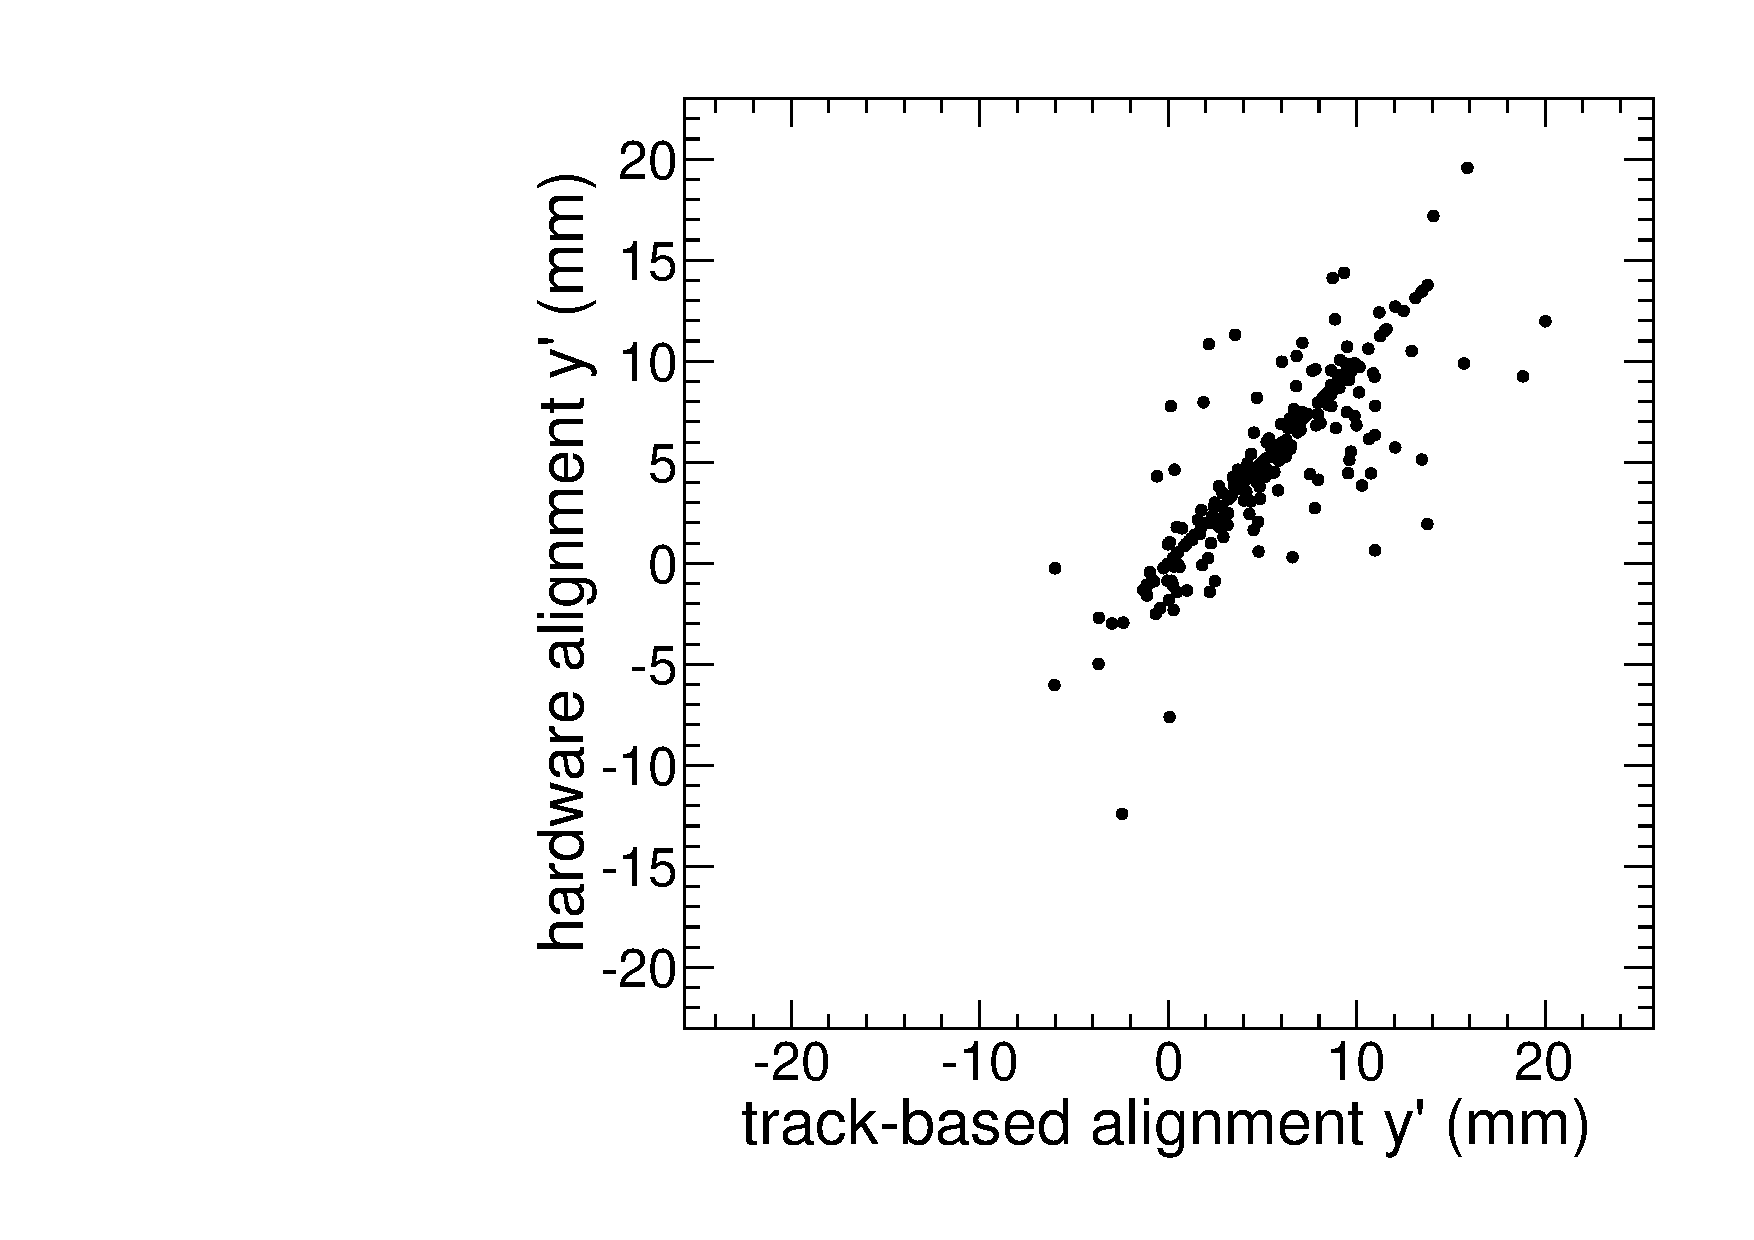
\includegraphics[width=0.33\linewidth]{hardware_y_corr.pdf}
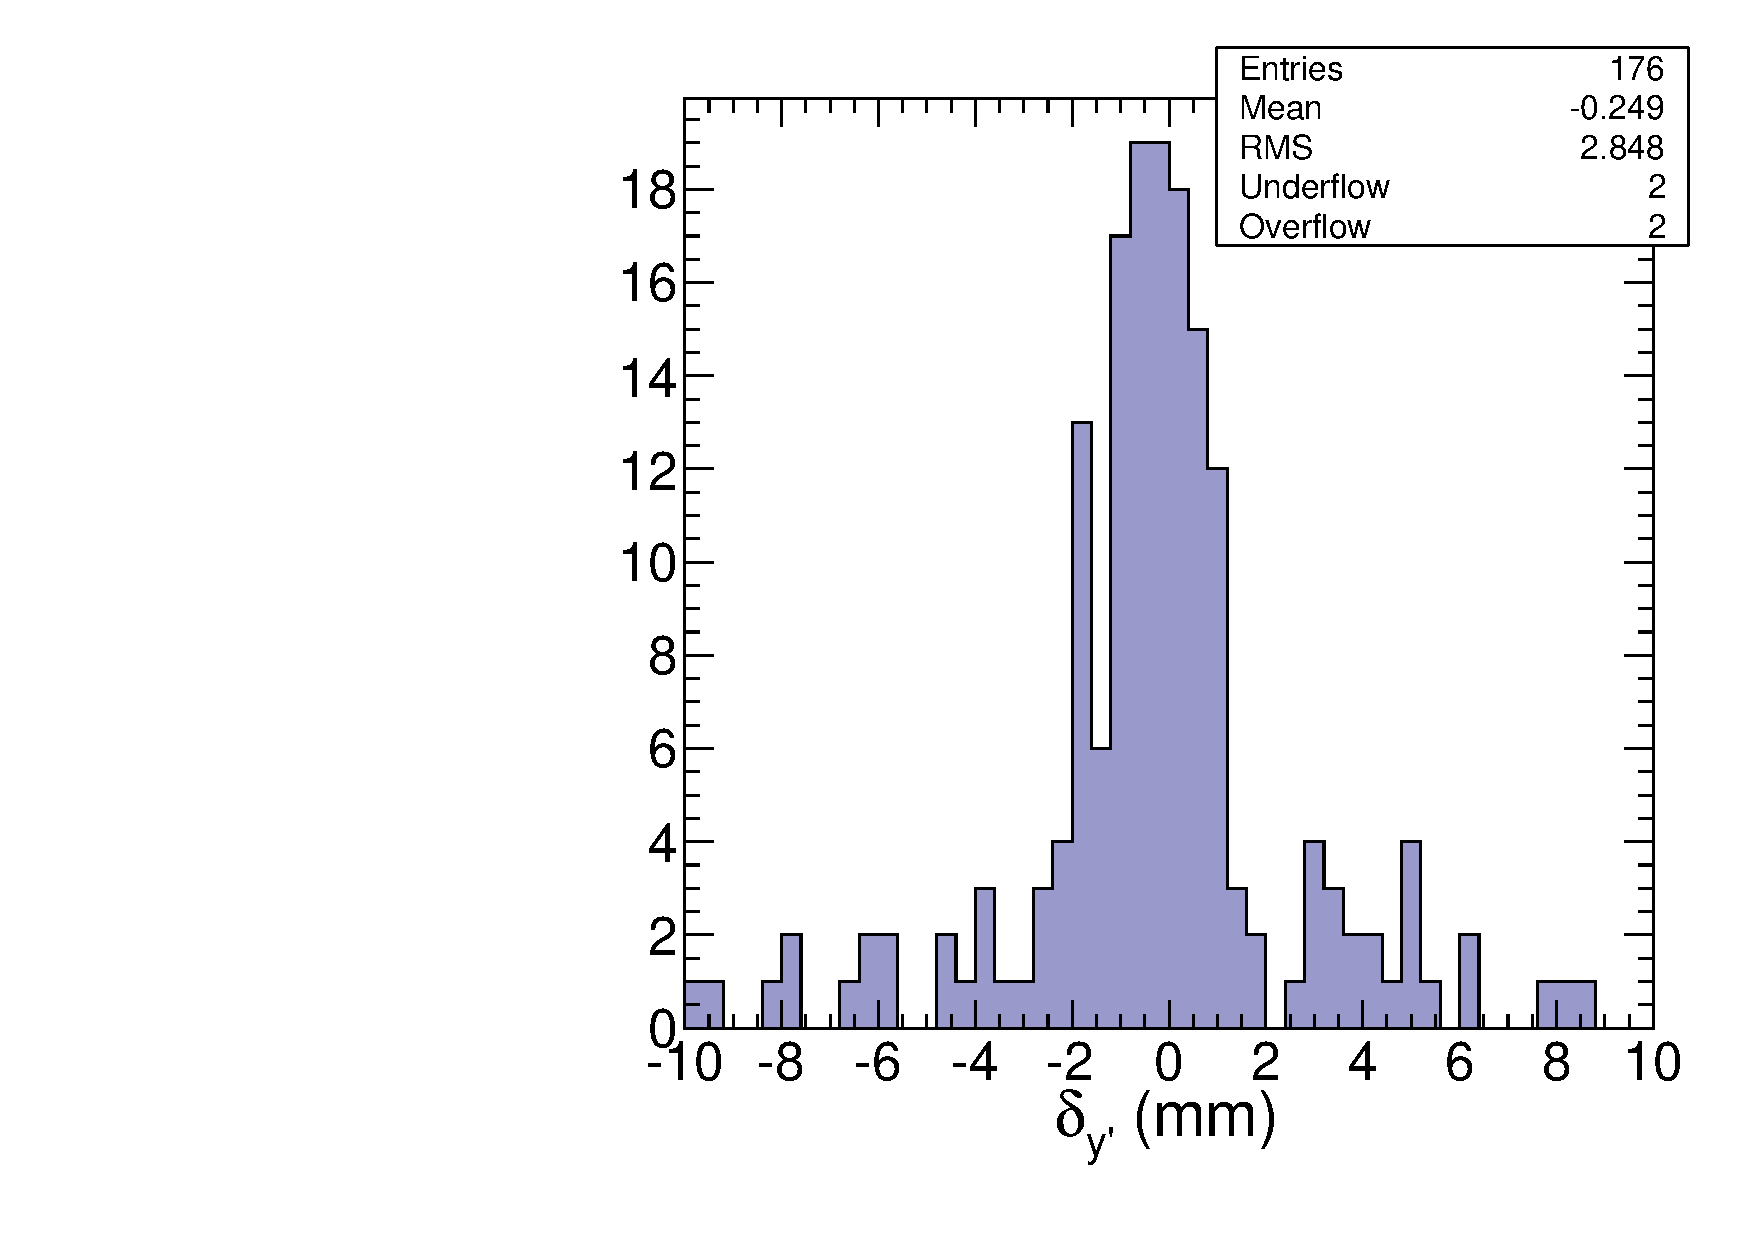
\includegraphics[width=0.33\linewidth]{hardware_y_diff.pdf}

\begin{itemize}
\item Track-based and hardware alignments {\it agree} for most
  chambers: central core width of about 1~mm or less in $x$, 2~mm in $y$

\item Different global positions, we should check GlobalPositionRcd
  (which will be updated next week)

\item Outliers listed below ($|x'| > 2$~mm): they might be the
  chambers that were not accessible to the hardware alignment
\end{itemize}

{\tiny
(wheel, station, sector): (-2, 1, 2) (-2, 1, 7) (-2, 1, 11) (-2, 1,
12) (-2, 2, 2) (-2, 2, 3) (-2, 2, 7) (-2, 3, 1) (-2, 3, 7) (0, 1, 12)
(2, 1, 1) (2, 1, 3) (2, 1, 6) (2, 2, 1) (2, 2, 5) (2, 3, 6) (-1, 4,
11) (2, 4, 6) (2, 4, 9)}
\end{frame}

\begin{frame}
\frametitle{Residuals quality}

A snapshot of the alignment quality browser for this alignment:

\only<1>{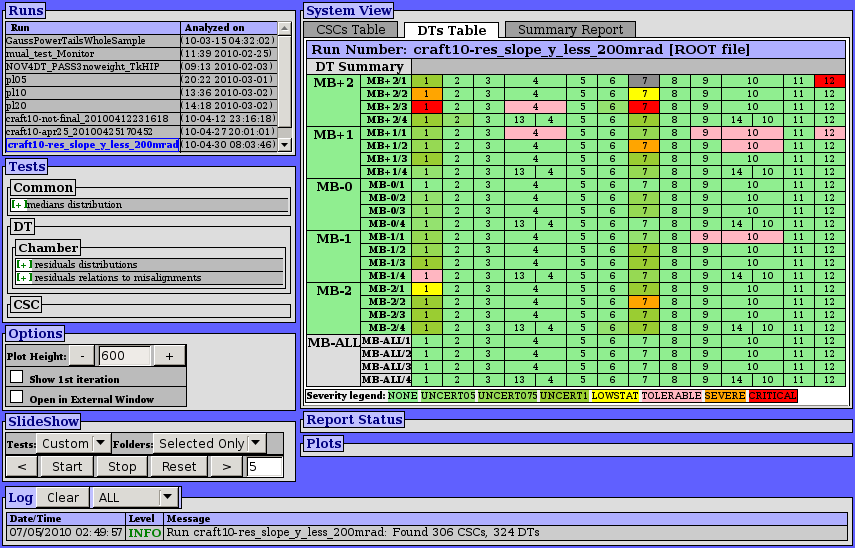
\includegraphics[width=\linewidth]{dt_table.png}} \only<2>{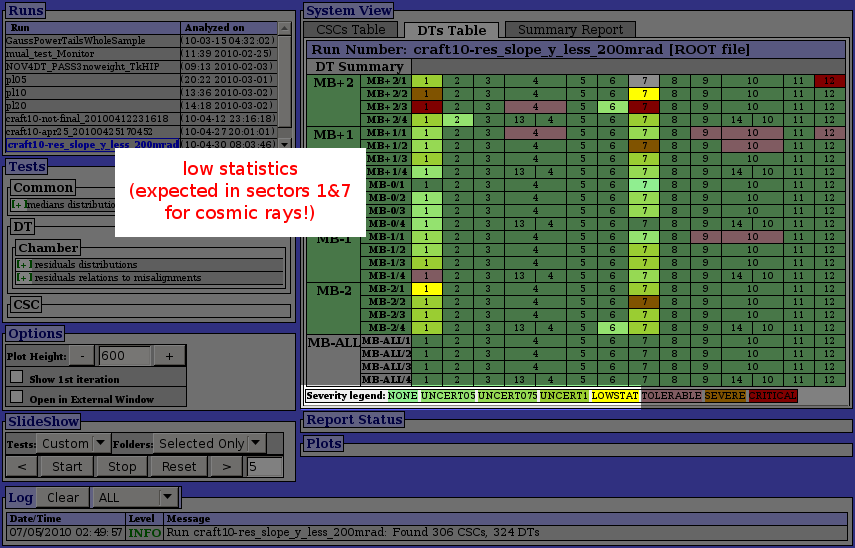
\includegraphics[width=\linewidth]{dt_table_0.png}} \only<3>{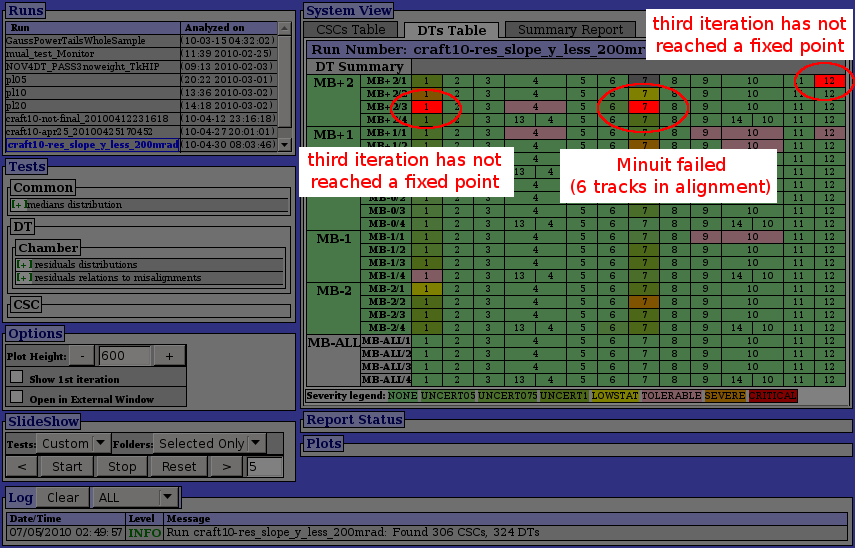
\includegraphics[width=\linewidth]{dt_table_1.png}} \only<4>{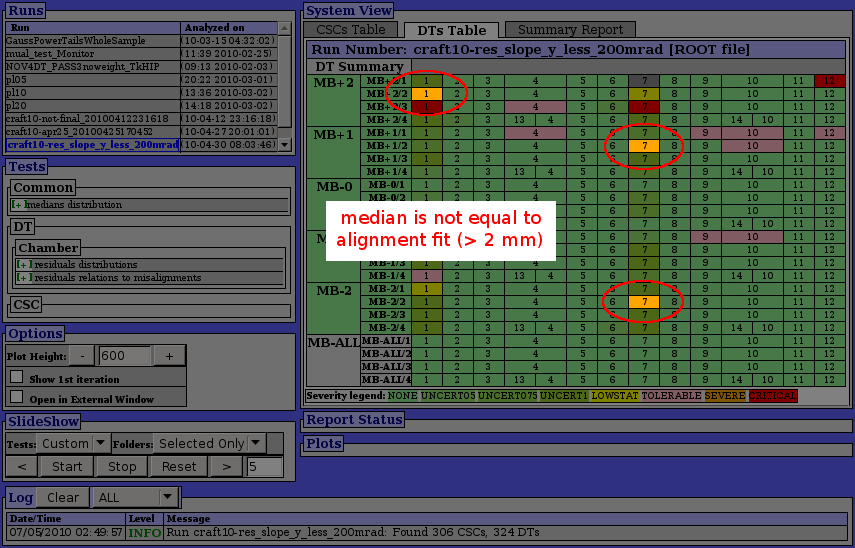
\includegraphics[width=\linewidth]{dt_table_2.png}} \only<5>{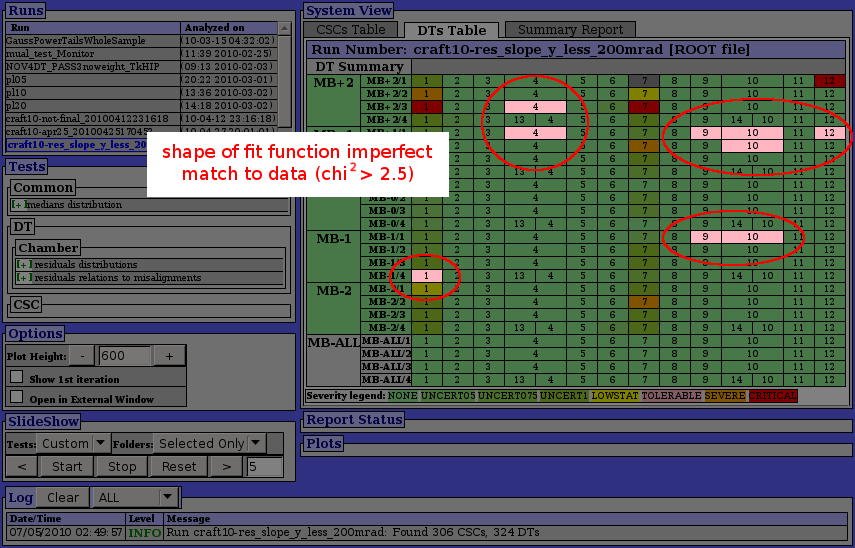
\includegraphics[width=\linewidth]{dt_table_3.png}}
\end{frame}

\begin{frame}
\frametitle{Residuals quality}

\begin{columns}
\column{0.6\linewidth}
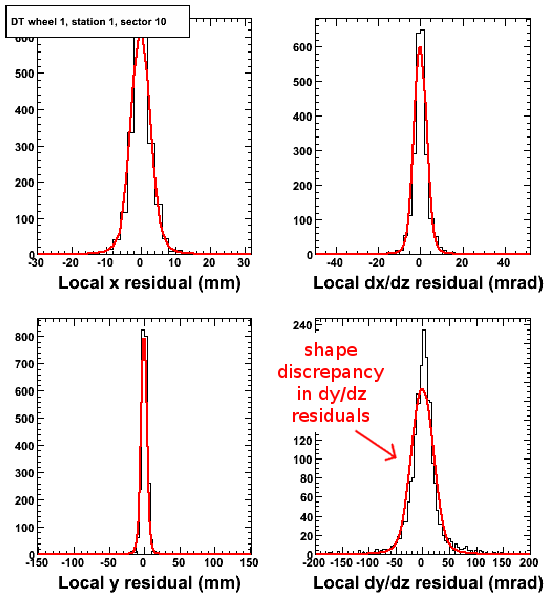
\includegraphics[width=\linewidth]{dt_table_4.png}

\column{0.4\linewidth}
\begin{itemize}
\item Selected one of the pink (tolerable) errors: a high-statistics
  chamber showing a shape discrepancy between fit and data

\item $\Delta \frac{dy}{dz}$ differs from general residuals shape

\item For now, truncating distribution at 200~mrad and not aligning
  corresponding parameter ($\Delta \frac{dy}{dz}$ corresponds to
  $\delta_{\phi_x}$)

\item Verified that applying this cut has negligible impact on the 4
  aligned parameters
\end{itemize}
\end{columns}
\end{frame}

\begin{frame}
\frametitle{Alignment strategy}

\begin{itemize}\setlength{\itemsep}{0.5 cm}
\item Procedure:
\begin{enumerate}\setlength{\itemsep}{0.1 cm}
\item start with hardware alignment
\item apply global position correction
\item replace hardware result with track-based if $|x_{\mbox{\tiny TB}} - x_{\mbox{\tiny HW}}| > 2 \sigma_{\mbox{\tiny TB}}$
\end{enumerate}

\item Step 3 is the ``motion policy'' recommended by our resolution projections note:
\begin{itemize}\setlength{\itemsep}{0.1 cm}
\item it guarantees that a superior prior geometry will not be
  replaced by statistical fluctuations in track-based alignment at the
  95\% confidence level

\item but clear track-based measurements of chamber misalignments
  {\it would} be corrected

\item more than half of the hardware constants are within $2
  \sigma_{\mbox{\tiny TB}}$ (after global position correction) and
  would be preserved in the final geometry
\end{itemize}
\end{itemize}
\end{frame}

%% \section*{First section}
%% \begin{frame}
%% \begin{center}
%% \Huge \textcolor{blue}{First section}
%% \end{center}
%% \end{frame}

\begin{frame}
\frametitle{Conclusions}

\begin{itemize}\setlength{\itemsep}{0.4 cm}
\item Reference-Target algorithm has been made more robust, but alignment results are unchanged

\item Physical displacement of DT chambers from 2009 $\to$ 2010 in $x$ is barely statistically significant

\item Most hardware and track-based results agree well, but there are enumerable outliers

\item Residuals in 2010 indicate what you'd expect: some problems related to low statistics in sectors 1\&7
\begin{itemize}
\item automated algorithm catches anomalies; we don't need to flip through thousands of plots
\end{itemize}

\item The ``motion policy'' publishes the best of a prior geometry and observed track-based measurements
\end{itemize}

\label{numpages}
\end{frame}

\end{document}
